\documentclass[color=black,device=normal,lang=cn,mode=geye]{elegantnote}
\usepackage{lecturenote}

\title{第3章笔记和习题}
\begin{document}
\maketitle
\section{行列式的构造(对应教材3.1节)}
下面通过一个简单的方法证明:
\begin{theorem}
    设 $A,B$ 是 $2$ 维列向量, 则平行四边形 $\Pi(A,B)$ 的有向面积 $v(\Pi(A,B))$ 为 $\det(A,B)$.
\end{theorem}
\begin{proof}
    图 \ref{f1} 可以说明 $v(\Pi(A,B))$ 具有以下的线性性质:
    \begin{enumerate}
        \item $\forall$ 纯量 $\lambda,v(\Pi(A,\lambda B))=v(\Pi(\lambda A,B))=\lambda v(\Pi(A,B))$,
        \item $\forall\ 2$ 维列向量 $C,v(\Pi(A,B+C))=v(\Pi(A,B))+v(\Pi(A,C))$,
        
        $v(\Pi(A+C,B))=v(\Pi(A,B))+v(\Pi(C,B))$.
    \end{enumerate}

    此外还有:
    \begin{enumerate}
        \item $\forall A\in\mathbb{R}^2,v(\Pi(A,A))=0$,
        \item $v(\Pi(E))=1$.
    \end{enumerate}

    设 $A=[a,b],B=[c,d]$, 由上述性质得
    \begin{align*}
        v(\Pi(A,B)) & =v(\Pi([a,b],[c,d])) \\
        & =v(\Pi([a,0],[c,0]))+v(\Pi([a,0],[0,d]))+v(\Pi([0,b],[c,0]))+v(\Pi([0,b],[0,d])) \\
        & =acv(\Pi([1,0],[1,0]))+adv(\Pi(E))+bcv(\Pi([0,1],[1,0]))+bdv(\Pi([0,1],[0,1])) \\
        & =adv(\Pi(E))+bcv(\Pi([0,1],[1,0])).
    \end{align*}

    $\because$
    \begin{align*}
        & v(\Pi(E))+v(\Pi([0,1],[1,0])) \\
        & =v(\Pi(E))+v(\Pi([0,1],[1,0]))+v(\Pi([1,0],[1,0]))+v(\Pi([0,1],[0,1])) \\
        & =v(\Pi([1,1],[1,1]))=0,
    \end{align*}

    $\therefore$
    \[v(\Pi(E))=-v(\Pi([0,1],[1,0])),\]
    \[v(\Pi(A,B))=(ad-bc)v(\Pi(E))=ad-bc.\qedhere\]
\end{proof}
\begin{figure}[htbp!]
    \centering
    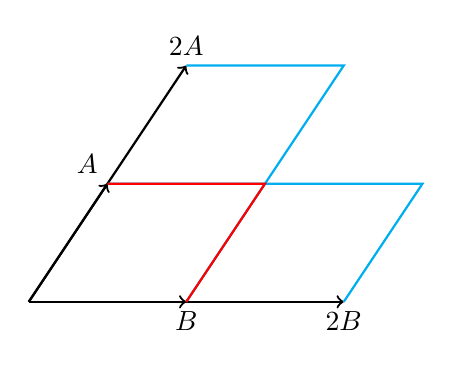
\begin{tikzpicture}[scale=.5]
        \draw [thick, ->] (0,0) -- (2,3);
        \node [above left] at (2,3) {$A$};
        \draw [thick, ->] (0,0) -- (4,0);
        \node [below] at (4,0) {$B$};
        \draw [thick, ->] (0,0) -- (4,6);
        \node [above] at (4,6) {$2A$};
        \draw [thick, ->] (0,0) -- (8,0);
        \node [below] at (8,0) {$2B$};
        \draw [thick, cyan] (8,0) -- (10,3) -- (2,3);
        \draw [thick, cyan] (4,0) -- (8,6) -- (4,6);
        \draw [thick, red] (4,0) -- (6,3) -- (2,3);
    \end{tikzpicture}
    \quad
    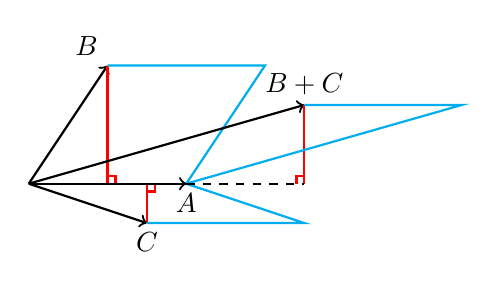
\begin{tikzpicture}[scale=.5]
        \draw [thick, ->] (0,2) -- (2,5);
        \draw [thick, red] (2,2) -- (2,5);
        \draw [thick, red] (2,2.2) -- (2.2,2.2) -- (2.2,2);
        \draw [thick, cyan] (2,5) -- (6,5) -- (4,2);
        \node [above left] at (2,5) {$B$};
        \draw [thick, ->] (0,2) -- (3,1);
        \draw [thick, red] (3,2) -- (3,1);
        \draw [thick, red] (3,1.8) -- (3.2,1.8) -- (3.2,2);
        \draw [thick, cyan] (3,1) -- (7,1) -- (4,2);
        \node [below] at (3,1) {$C$};
        \draw [thick, ->] (0,2) -- (7,4);
        \draw [thick, red] (7,4) -- (7,2);
        \draw [thick, red] (7,2.2) -- (6.8,2.2) -- (6.8,2);
        \draw [thick, cyan] (7,4) -- (11,4) -- (4,2);
        \node [above] at (7,4) {$B+C$};
        \draw [thick, ->] (0,2) -- (4,2);
        \draw [thick, dashed] (4,2) -- (7,2);
        \node [below] at (4,2) {$A$};
    \end{tikzpicture}
    \caption{有向面积的线性性质. 左图对应性质 1, 右图对应性质 2}\label{f1}
\end{figure}

由于证明过程中只涉及 $v(\Pi(A,B))$ 的一些性质, 因此这一证明很容易推广到 $n$ 维的情形.

设 $A\in M_n(\mathbb{R})=(A^{(1)},A^{(2)},\cdots,A^{(n)})$, 函数 $\det:M_n(\mathbb{R})\to\mathbb{R}$ 满足下列性质:
\begin{property}\label{p1}
    $\det$ 对 $A$ 的行或列是多重线性的(下面只讨论列的情况, 行的情况类似).
\end{property}
\begin{property}\label{p2}
    $\det$ 对 $A$ 的行或列是斜对称的.
\end{property}
\begin{property}\label{p3}
    $\det(\varepsilon^1,\varepsilon^2,\cdots,\varepsilon^n)=1$.
\end{property}
从性质 \ref{p2} 可以得到一个推论:
\begin{corollary}\label{c1}
    若 $A$ 中有两个行或列向量相等, 则 $\det A=0$.
\end{corollary}
\begin{proof}
    只讨论列的情况, 行的情况类似.

    设 $A^{(i)}=A^{(j)}$. 由性质 \ref{p1},
    \begin{align*}
        & \det(A^{(1)},\cdots,A^{(i)},\cdots,A^{(j)},\cdots,A^{(n)})=-\det(A^{(1)},\cdots,A^{(j)},\cdots,A^{(i)},\cdots,A^{(n)}) \\
        & \Rightarrow2\det(A^{(1)},\cdots,A^{(i)},\cdots,A^{(i)},\cdots,A^{(n)})=0 \\
        & \Rightarrow\det(A^{(1)},\cdots,A^{(i)},\cdots,A^{(j)},\cdots,A^{(n)})=0 \\
        & \Rightarrow\det A=0.\qedhere
    \end{align*}
\end{proof}
\begin{corollary}\label{c2}
    $\forall\sigma\in S_n$,
    \[\det(A^{(\sigma(1))},A^{(\sigma(2))},\cdots,A^{(\sigma(n))})=\varepsilon_\sigma\det A,\]

    其中 $\varepsilon_\sigma$ 是 $\sigma$ 的符号.
\end{corollary}
\begin{proof}
    将 $\sigma$ 写成对换的乘积:
    \[\sigma=\sigma_1\sigma_2\cdots\sigma_k,\]

    由性质 \ref{p2} 得对于任意的向量 $B^{(1)},B^{(2)},\cdots,B^{(n)}$ 和对换 $\sigma_i$, 都有
    \[\det(B^{(\sigma_i(1))},B^{(\sigma_i(2))},\cdots,B^{(\sigma_i(n))})=-\det(B^{(1)},B^{(2)},\cdots,B^{(n)}),\]

    $\therefore$
    \begin{align*}
        & \det\left(A^{(\sigma(1))},A^{(\sigma(2))},\cdots,A^{(\sigma(n))}\right) \\
        & =\det\left(A^{(\sigma_1\sigma_2\cdots\sigma_k(1))},A^{(\sigma_1\sigma_2\cdots\sigma_k(2))},\cdots,A^{(\sigma_1\sigma_2\cdots\sigma_k(n))}\right) \\
        & =(-1)\det\left(A^{(\sigma_1\sigma_2\cdots\sigma_{k-1}(1))},A^{(\sigma_1\sigma_2\cdots\sigma_{k-1}(2))},\cdots,A^{(\sigma_1\sigma_2\cdots\sigma_{k-1}(n))}\right) \\
        & =(-1)^2\det\left(A^{(\sigma_1\sigma_2\cdots\sigma_{k-2}(1))},A^{(\sigma_1\sigma_2\cdots\sigma_{k-2}(2))},\cdots,A^{(\sigma_1\sigma_2\cdots\sigma_{k-2}(n))}\right) \\
        & =\cdots \\
        & =(-1)^k\det(A^{(1)},A^{(2)},\cdots,A^{(n)}) \\
        & =\varepsilon_\sigma\det A.\qedhere
    \end{align*}
\end{proof}

设 $A^{(j)}=[a_{1j},a_{2j},\cdots,a_{nj}]$, 则
\[A^{(j)}=\sum\limits_{i=1}^na_{ij}E^{(i)},\]

其中 $E^{(i)}=[\underbrace{0,\cdots,0}_{i-1\text{个}0},1,\underbrace{0,\cdots,0}_{n-i\text{个}0}]$. $\therefore$
\begin{align*}
    \det(A) & =\det(A^{(1)},A^{(2)},\cdots,A^{(n)}) \\
    & =\det\left(\sum\limits_{i=1}^na_{i1}E^{(i)},\sum\limits_{i=1}^na_{i2}E^{(i)},\cdots,\sum\limits_{i=1}^na_{in}E^{(i)}\right).
\end{align*}

由推论 \ref{c1},
\begin{align*}
    & \det\left(\sum\limits_{i=1}^na_{i1}E^{(i)},\sum\limits_{i=1}^na_{i2}E^{(i)},\cdots,\sum\limits_{i=1}^na_{in}E^{(i)}\right) \\
    & =\sum\limits_{i_1=1}^n\sum\limits_{i_2=1}^n\cdots\sum\limits_{i_n=1}^na_{i_11}a_{i_22}\cdots a_{i_nn}\det\left(E^{(i_1)},E^{(i_2)},\cdots,E^{(i_n)}\right). \\
\end{align*}

由性质 \ref{p2}, $i_1,i_2,\cdots,i_n$ 互不相同. $\therefore$
\[\det A=\sum\limits_{\sigma\in S_n}a_{\sigma(1),1}a_{\sigma(2),2}\cdots a_{\sigma(n),n}\det\left(E^{(\sigma(1))},E^{(\sigma(2))},\cdots,E^{(\sigma(n))}\right),\]

其中 $S_n$ 是 $n$ 元置换的全体.

由推论 \ref{c2} 得 $\det\left(E^{(\sigma(1))},E^{(\sigma(2))},\cdots,E^{(\sigma(n))}\right)=\varepsilon_\sigma\det E=\varepsilon_\sigma$, $\therefore$
\begin{equation}\label{eq1.1}
    \det A=\sum\limits_{\sigma\in S_n}\varepsilon_\sigma a_{\sigma(1),1}a_{\sigma(2),2}\cdots a_{\sigma(n),n}.
\end{equation}

由书上的定理 1, 这里的展开式与书上的是一致的.

由式 (\ref{eq1.1}), 行列式的每一项中每一行和每一列都只出现一个元素.

满足性质 \ref{p1}, \ref{p2}, \ref{p3} 的函数一定具有式 (\ref{eq1.1}) 的形式(如果我们用式 (\ref{eq1.1}) 来定义行列式, 那么称这三个性质\textbf{完全确定了}行列式). 事实上由式 (\ref{eq1.1}) 也可以推出前面的三个性质(也就是说式 (\ref{eq1.1}) 与这三个性质等价).
\begin{theorem}
    如果用式 (\ref{eq1.1}) 定义行列式, 那么 $\det$ 满足性质 \ref{p1}, \ref{p2}, \ref{p3}.
\end{theorem}
\begin{proof}
    对于性质 \ref{p1}, 下面只讨论行的情况, 列的情况类似.

    设 $A=[A_{(1)},A_{(2)},\cdots,A_{(k)},\cdots,A_{(n)}]=(a_{ij})$, 其中
    \[A_{(k)}=\alpha A_{(k)}'+\beta A_{(k)}'',\]
    \[A_{(k)}'=(a'_{k1},a'_{k2},\cdots,a'_{kn}),\quad A_{(k)}''=(a''_{k1},a''_{k2},\cdots,a''_{kn}),\]

    由定理 1, 式 (\ref{eq1.1}) 等价于
    \[\det A=\sum\limits_{\sigma\in S_n}\varepsilon_\sigma a_{1,\sigma(1)}a_{2,\sigma(2)}\cdots a_{n,\sigma(n)}.\]

    $\because a_{kj}=\alpha a_{kj}'+\beta a_{kj}'',\therefore$
    \begin{align*}
        & \sum\limits_{\sigma\in S_n}\varepsilon_\sigma a_{1,\sigma(1)}a_{2,\sigma(2)}\cdots a_{n,\sigma(n)} \\
        = & \ \sum\limits_{\sigma\in S_n}\varepsilon_\sigma a_{1,\sigma(1)}\cdots a_{k-1,\sigma(k-1)}(\alpha a_{k,\sigma(k)}'+\beta a_{k,\sigma(k)}'')a_{k+1,\sigma(k+1)}\cdots a_{n,\sigma(n)} \\
        = & \ \alpha\sum\limits_{\sigma\in S_n}\varepsilon_\sigma a_{1,\sigma(1)}\cdots a_{k-1,\sigma(k-1)}a_{k,\sigma(k)}'a_{k+1,\sigma(i+1)}\cdots a_{n,\sigma(n)} \\
        & +\beta\sum\limits_{\sigma\in S_n}\varepsilon_\sigma a_{1,\sigma(1)}\cdots a_{k-1,\sigma(k-1)}a_{k,\sigma(k)}''a_{k+1,\sigma(k+1)}\cdots a_{n,\sigma(n)} \\
        = & \ \alpha\det(A_{(1)},A_{(2)},\cdots,A'_{(k)},\cdots,A_{(n)})+\beta\det(A_{(1)},A_{(2)},\cdots,A''_{(k)},\cdots,A_{(n)}).
    \end{align*}

    对于性质 \ref{p2}, 下面只讨论行的情况, 列的情况类似.

    设
    \[A=[A_{(1)},\cdots,A_{(k)},\cdots,A_{(l)},\cdots,A_{(n)}]=(a_{ij}),A'=[A_{(1)},\cdots,A_{(l)},\cdots,A_{(k)},\cdots,A_{(n)}]\]

    设 $\tau=(k,l)$, 则 $A'=(a_{\tau(j),j})$. $\therefore$
    \[\det A'=\sum\limits_{\sigma\in S_n}\varepsilon_\sigma a_{\sigma\tau(1),1}a_{\sigma\tau(2),2}\cdots a_{\sigma\tau(n),n}.\]

    令 $\pi=\sigma\tau$, 则 $\sigma=\pi\tau,\varepsilon_\pi=\varepsilon_\sigma\varepsilon_\tau=-\varepsilon_\sigma$,
    \[\det A'=\sum\limits_{\pi\tau\in S_n}-\varepsilon_\pi a_{\pi(1),1}a_{\pi(2),2}\cdots a_{\pi(n),n}.\]

    $\because$ 映射
    \[\begin{array}{rcl}
        S_n & \to & S_n \\
        \pi & \to & \pi\tau
    \end{array}\]

    是双射, $\therefore$
    \begin{align*}
        \det A' & =\sum\limits_{\pi\in S_n}-\varepsilon_\pi a_{\pi(1),1}a_{\pi(2),2}\cdots a_{\pi(n),n} \\
        & =-\sum\limits_{\pi\in S_n}\varepsilon_\pi a_{\pi(1),1}a_{\pi(2),2}\cdots a_{\pi(n),n} \\
        & =-\det A.
    \end{align*}

    对于性质 \ref{p3}, $\because E=(\delta_{ij})$, 其中 $\delta_{ij}$ 是 Kronecker $\delta$ 函数, $\therefore$
    \[\det A=\sum\limits_{\sigma\in S_n}\varepsilon_\sigma\prod\limits_{i=1}^n\delta_{i,\sigma(i)}.\]

    $\because\prod\limits_{i=1}^n\delta_{i,\sigma(i)}\neq0$ 当且仅当 $\sigma=e$, 其中 $e$ 是恒等置换, $\therefore$
    \[\sum\limits_{\sigma\in S_n}\varepsilon_\sigma\prod\limits_{i=1}^n\delta_{i,\sigma(i)}=\varepsilon_e\prod\limits_{i=1}^n\delta_{ii}=1.\qedhere\]
\end{proof}
\section{行列式的性质(对应教材3.2节)}
设
\[A=\begin{pmatrix}
    a_{11} & \cdots & a_{1,j-1} & 0 & a_{1,j+1} & \cdots & a_{1n} \\
    \vdots && \vdots & \vdots & \vdots && \vdots \\
    a_{i-1,1} & \cdots & a_{i-1,j-1} & 0 & a_{i-1,j+1} & \cdots & a_{i-1,n} \\
    a_{i1} & \cdots & a_{i,j-1} & a_{ij} & a_{i,j+1} & \cdots & a_{in} \\
    a_{i+1,1} & \cdots & a_{i+1,j-1} & 0 & a_{i+1,j+1} & \cdots & a_{i+1,n} \\
    \vdots && \vdots & \vdots & \vdots && \vdots \\
    a_{n1} & \cdots & a_{n,j-1} & 0 & a_{n,j+1} & \cdots & a_{nn} \\
\end{pmatrix}.\]

书上的定理 1 的证明中有这样的等式:
\[\det A=(-1)^j\begin{vmatrix}
    0 & a_{11} & \cdots & a_{1,j-1} & a_{1,j+1} & \cdots & a_{1n} \\
    \vdots && \vdots & \vdots & \vdots && \vdots \\
    0 & a_{i-1,1} & \cdots & a_{i-1,j-1} & a_{i-1,j+1} & \cdots & a_{i-1,n} \\
    a_{ij} & a_{i1} & \cdots & a_{i,j-1} & a_{i,j+1} & \cdots & a_{in} \\
    0 & a_{i+1,1} & \cdots & a_{i+1,j-1} & a_{i+1,j+1} & \cdots & a_{i+1,n} \\
    \vdots && \vdots & \vdots & \vdots && \vdots \\
    0 & a_{n1} & \cdots & a_{n,j-1} & a_{n,j+1} & \cdots & a_{nn} \\
\end{vmatrix},\]

这等价于
\[\det A=(-1)^j\det(A^{(i)},A^{(1)},\cdots,A^{(i-1)},A^{(i+1)},\cdots,A^{(n)}).\]

考察循环 $(i\ i-1\ \cdots\ 2\ 1)$, 由推论 \ref{c2} 得上式成立.

书上的定理 3 有另一种证明方法. 先证明一个引理.
\begin{lemma}\label{l2.1}
    矩阵 $A\in M_n(\mathbb{R})$ 的行或列线性相关 $\Rightarrow\det A=0$.
\end{lemma}
\begin{proof}
    设 $A_{(i)}=\sum\limits_{k=1}^n\lambda_kA_{(k)}$. 设 $A'=\prod\limits_{k=1}^nF_{i,k}(-\lambda_{k})A$, 则 $A'_{(i)}=0$. 由行列式的性质 D5 得 $\det A'=0$. 由行列式的性质 D7 得 $\det A=\det A'=0.$
\end{proof}
\begin{theorem}[书上的定理 3]
    设 $A,B$ 是 $n$ 阶方阵, 则
    \[\det AB=\det A\det B.\]
\end{theorem}
\begin{proof}
    (a) 若 $A$ 退化或 $B$ 退化, 由 2.3 节的定理 3 得 $AB$ 退化. 由引理 \ref{l2.1} $\det A=0\vee\det B=0,\det AB=0$, 有
    \[\det AB=\det A\det B.\]

    (b) 若 $A,B$ 都非退化, 设分别对 $A,B$ 进行初等行变换, 初等列变换得到
    \[A'=\begin{pmatrix}
        a_{1} \\
        & a_{2} \\
        && \ddots \\
        &&& a_{n} \\
    \end{pmatrix},\quad B'=\begin{pmatrix}
        b_{1} \\
        & b_{2} \\
        && \ddots \\
        &&& b_{n} \\
    \end{pmatrix},\]

    有
    \[A=P_1P_2\cdots P_sA',\quad B=B'Q_1Q_2\cdots Q_t,\]
    \[\det A=(-1)^p\det A',\quad\det B=(-1)^q\det B',\]
    \[\det A'B'=\det A'\det B',\]

    其中 $P_i,Q_j\ (i=1,2,\cdots,s,j=1,2,\cdots,t)$ 是初等矩阵, $p,q$ 是常数.

    $\therefore$
    \[AB=P_1P_2\cdots P_sA'B'Q_1Q_2\cdots Q_t,\]
    \[\det AB=(-1)^{p+q}\det A'B'=\det A\det B.\qedhere\]
\end{proof}
\section{行列式的应用(对应教材3.3节)}
可以不用伴随矩阵得到 Crammer 公式.
\begin{theorem}[书上的定理 2]
    若线性方程组 $AX=B$ 有解 $X_0=[x_1,x_2,\cdots,x_n]$, 则 $x_i=\dfrac{\det D_i}{\det A}$, 其中 $D_i=(A^{(1)},A^{(2)},\cdots,A^{(i-1)},B,A^{(i+1)},\cdots,A^{(n)})$.
\end{theorem}
\begin{proof}    
    有
    \[B=x_1A^{(1)}+x_2A^{(2)}+\cdots+x_nA^{(n)}=(A^{(1)},A^{(2)},\cdots,A^{(n)})X_0.\]

    $\therefore$
    \begin{align*}
        \det D_i & =\det\left(A^{(1)},A^{(2)},\cdots,A^{(i-1)},B,A^{(i+1)},\cdots,A^{(n)}\right) \\
        & =\det\left(A^{(1)},A^{(2)},\cdots,A^{(i-1)},\sum\limits_{j=1}^nx_jA^{(j)},A^{(i+1)},\cdots,A^{(n)}\right) \\
        & =\sum\limits_{j=1}^nx_j\det\left(A^{(1)},A^{(2)},\cdots,A^{(i-1)},A^{(j)},A^{(i+1)},\cdots,A^{(n)}\right) \\
        & =x_i\det\left(A^{(1)},A^{(2)},\cdots,A^{(i-1)},A^{(i)},A^{(i+1)},\cdots,A^{(n)}\right) \\
        & =x_i\det A.
    \end{align*}

    $\because AX=B$ 有解, $\therefore\det A\neq0$. $\therefore x_i=\dfrac{\det D_i}{\det A}$.
\end{proof}

书上的命题 4.21 和 4.22 写得不是很清楚. 这里补充一下. 先证明一个引理.
\begin{lemma}\label{l3.1}
    设 $m\leq n$,
    \begin{align*}
        A^{(1)} & =[a_{11},\cdots,a_{n1}], & A^{(2)} & =[a_{12},\cdots,a_{n2}], & \cdots && A^{(n)} & =[a_{1n},\cdots,a_{nn}]\in\mathbb{R}^n, \\
        \widetilde{A}^{(1)} & =[a_{11},\cdots,a_{m1}], & \widetilde{A}^{(2)} & =[a_{12},\cdots,a_{m2}], & \cdots && \widetilde{A}^{(n)} & =[a_{1n},\cdots,a_{mn}]\in\mathbb{R}^m.
    \end{align*}
    
    如果 $\widetilde{A}^{(1)},\widetilde{A}^{(2)},\cdots,\widetilde{A}^{(n)}$ 线性无关, 那么 $A^{(1)},A^{(2)},\cdots,A^{(n)}$ 线性无关.
\end{lemma}
\begin{proof}
    证明逆否命题. $\because A^{(1)},A^{(2)},\cdots,A^{(n)}$ 线性相关, $\therefore$ 方程组
    \[\begin{cases}
        a_{11}x_1+a_{12}x_2+\cdots+a_{1n}x_n=0 \\
        a_{21}x_1+a_{22}x_2+\cdots+a_{2n}x_n=0 \\
        \cdots \\
        a_{n1}x_1+a_{n2}x_2+\cdots+a_{nn}x_n=0 \\
    \end{cases}\]
    有非零解. 这个解也是方程组
    \[\begin{cases}
        a_{11}x_1+a_{12}x_2+\cdots+a_{1n}x_n=0 \\
        a_{21}x_1+a_{22}x_2+\cdots+a_{2n}x_n=0 \\
        \cdots \\
        a_{m1}x_1+a_{m2}x_2+\cdots+a_{mn}x_n=0 \\
    \end{cases}\]
    的解. $\therefore\widetilde{A}^{(1)},\widetilde{A}^{(2)},\cdots,\widetilde{A}^{(n)}$ 线性相关.
\end{proof}
\begin{theorem}[书上的命题 4.21]\label{t3.2}
    $m\times n$ 矩阵 $A=(a_{ij})$ 的秩 $r$ 等于 $A$ 的非零子式的阶数中的最大者.
\end{theorem}
\begin{proof}
    $\because A$ 的秩为 $r$, $\therefore A$ 有 $r$ 行 $A_{(i_1)},A_{(i_2)},\cdots,A_{(i_r)}$ 线性无关. 考虑 $r\times n$ 矩阵
    \[A'=(A_{(i_1)},A_{(i_2)},\cdots,A_{(i_r)}).\]

    $\because A'$ 有 $r$ 行线性无关, $\therefore A'$ 的秩为 $r$. 由书上的引理 4.20 得 $A'$ 有一个 $r$ 阶子式不为 $0$.
    
    $\because A'$ 的子式也是 $A$ 的子式, $\therefore A$ 有一个 $r$ 阶子式不为 $0$. $\therefore r\leq A$ 的非零子式的阶数中的最大者.

    如果 $A$ 有一个 $s$ 阶子式 $M\begin{pmatrix} i_1 & \cdots & i_s \\ j_1 & \cdots & j_s \end{pmatrix}$ 不为 $0$, 由书上的定理 4.17 得向量组
    \[[a_{i_1j_1},a_{i_2j_1},\cdots,a_{i_sj_1}],\quad[a_{i_1j_2},a_{i_2j_2},\cdots,a_{i_sj_2}],\quad\cdots,\quad[a_{i_1j_n},a_{i_2j_n},\cdots,a_{i_sj_n}]\]
    线性无关. 由引理 \ref{l3.1} 得 $A^{(j_1)},A^{(j_2)},\cdots,A^{(j_n)}$ 线性无关. $\therefore r\geq s$. $\because$ 这对 $A$ 的任意的子式都成立, $\therefore r\geq A$ 的非零子式的阶数中的最大者.
\end{proof}
\begin{theorem}[书上的命题 4.22]
    假设一个 $m\times n$ 矩阵 $A=(a_{ij})$ 的某个子式 $M\begin{pmatrix} i_1 & \cdots & i_r \\ j_1 & \cdots & j_r \end{pmatrix}$ 非零, 但这个子式的任何上级都是 $0$, 那么 $\rank A=r$.
\end{theorem}
\begin{proof}
    与定理 \ref{t3.2} 的证明类似, 得 $\rank A\geq r$.

    设 $M\begin{pmatrix} i_1 & \cdots & i_r \\ j_1 & \cdots & j_r \end{pmatrix}$ 的某个上级为 $M\begin{pmatrix} i_1 & \cdots & i_r & i_s \\ j_1 & \cdots & j_r & j_t \end{pmatrix}$, 有
    \[\begin{vmatrix}
        a_{i_1j_1} & a_{i_1j_2} & \cdots & a_{i_1j_r} & a_{i_1j_t} \\
        a_{i_2j_1} & a_{i_2j_2} & \cdots & a_{i_2j_r} & a_{i_2j_t} \\
        \vdots & \vdots & \ddots & \vdots & \vdots \\
        a_{i_rj_1} & a_{i_rj_2} & \cdots & a_{i_rj_r} & a_{i_rj_t} \\
        a_{i_sj_1} & a_{i_sj_2} & \cdots & a_{i_sj_r} & a_{i_sj_t} \\
    \end{vmatrix}=0.\]

    按最后一行展开, 得
    \begin{equation}\label{eq3.1}
        a_{i_sj_1}M_1+a_{i_sj_2}M_2+\cdots+a_{i_sj_r}M_r+a_{i_sj_t}M\begin{pmatrix}
            i_1 & \cdots & i_{r-1} & j_r \\
            j_1 & \cdots & j_{r-1} & j_r
        \end{pmatrix}=0,
    \end{equation}

    其中
    \[M_u=(-1)^{(r+1)+u}\begin{pmatrix}
        i_2 & \cdots & \hat{i}_u & \cdots & i_r & j_t \\
        j_2 & \cdots & \hat{j}_u & \cdots & j_r & j_t
    \end{pmatrix}\quad(u=1,2,\cdots,r)\]
    (加`` $\hat{}$ ''表示只去掉这一元素, 比如 $1,\cdots,\hat{i},\cdots,n$ 表示 $1,\cdots,i-1,i+1,\cdots,n$).
    
    设 $v=1,2,\cdots,r$, 将 $M\begin{pmatrix} i_1 & \cdots & i_r & i_s \\ j_1 & \cdots & j_r & j_t \end{pmatrix}$ 对应的子阵的最后一行替换为第 $i_v$ 行得到的矩阵为 $M_{(v)}$. $\because M_{(v)}$ 有两行相等, 由行列式的性质 D6 得 $\det M_{(v)}=0$. 按最后一行展开 $M_{(v)}$, 得
    \[a_{i_vj_1}M_1+a_{i_vj_2}M_2+\cdots+a_{i_vj_r}M_r+a_{i_vj_t}M\begin{pmatrix}
        i_1 & \cdots & i_{r-1} & j_r \\
        j_1 & \cdots & j_{r-1} & j_r
    \end{pmatrix}=0.\]

    $\because$ 上式对任意的 $v=1,\cdots,r$ 都成立, 式 (\ref{eq3.1}) 对任意的 $i_s\in\{1,\cdots,m\}\backslash\{i_1,\cdots,i_r\}$ 都成立, $\therefore\forall i=1,2,\cdots,m$, 有
    \[a_{ij_1}M_1+a_{ij_2}M_2+\cdots+a_{ij_r}M_r+a_{ij_t}M\begin{pmatrix}
        i_1 & \cdots & i_{r-1} & j_r \\
        j_1 & \cdots & j_{r-1} & j_r
    \end{pmatrix}=0.\]

    $\therefore$
    \[M_1A^{(j_1)}+M_2A^{(j_2)}+\cdots+M_rA^{(j_r)}+M\begin{pmatrix}
        i_1 & \cdots & i_{r-1} & j_r \\
        j_1 & \cdots & j_{r-1} & j_r
    \end{pmatrix}A^{(j_t)}=0.\]

    $\because M\begin{pmatrix} i_1 & \cdots & i_{r-1} & j_r \\ j_1 & \cdots & j_{r-1} & j_r \end{pmatrix}\neq0$, $\therefore$
    \[A^{(j_t)}=-\dfrac{M_1}{M\begin{pmatrix}
        i_1 & \cdots & i_{r-1} & j_r \\
        j_1 & \cdots & j_{r-1} & j_r
    \end{pmatrix}}A^{(j_1)}-\cdots-\dfrac{M_r}{M\begin{pmatrix}
        i_1 & \cdots & i_{r-1} & j_r \\
        j_1 & \cdots & j_{r-1} & j_r
    \end{pmatrix}}A^{(j_r)}.\]

    $\therefore A^{(j_t)}$ 是 $A^{(j_1)},A^{(j_2)},\cdots,A^{(j_r)}$ 的线性组合. 这对 $\forall j_t\in\{1,2,\cdots,n\}\backslash\{j_1,j_2,\cdots,j_r\}$ 都成立, $\therefore A$ 的列空间的维数 $\leq r$. $\therefore\rank A\leq r$.
\end{proof}
\section{行列式的公理化构造(对应教材3.4节)}
下面证明第二公理化构造第一公理化构造是等价的. 从第一公理化构造推出第二公理化构造是显然的, $\therefore$ 只需证明从第二公理化构造的 3 条公理(书上的公理 2.1, 公理 2.2, 公理 2.3)可以推出第一公理化构造的 3 条公理(书上的公理 1.1, 公理 1.2, 公理 1.3).
\begin{lemma}\label{l4.1}
    (II) 型初等行变换不改变 $\mathcal{D}$ 的值.
\end{lemma}
\begin{proof}
    考察
    \[\mathcal{D}(A_{(1)},\cdots,A_{(i)}+\lambda A_{(j)},\cdots,A_{(j)},\cdots,A_{(n)})\ (\lambda\neq0).\]

    由书上的公理 2.1,
    \[\mathcal{D}(A_{(1)},\cdots,A_{(i)},\cdots,A_{(j)},\cdots,A_{(n)})=\lambda^{-1}\mathcal{D}(A_{(1)},\cdots,A_{(i)},\cdots,\lambda A_{(j)},\cdots,A_{(n)}).\]

    由书上的公理 2.2,
    \begin{align*}
        & \lambda^{-1}\mathcal{D}(A_{(1)},\cdots,A_{(i)},\cdots,\lambda A_{(j)},\cdots,A_{(n)}) \\
        & =\lambda^{-1}\mathcal{D}(A_{(1)},\cdots,A_{(i)}+\lambda A_{(j)},\cdots,\lambda A_{(j)},\cdots,A_{(n)}).
    \end{align*}

    由书上的公理 2.1,
    \begin{align*}
        & \lambda^{-1}\mathcal{D}(A_{(1)},\cdots,A_{(i)}+\lambda A_{(j)},\cdots,\lambda A_{(j)},\cdots,A_{(n)}) \\
        & =\mathcal{D}(A_{(1)},\cdots,A_{(i)}+\lambda A_{(j)},\cdots,A_{(j)},\cdots,A_{(n)}).
    \end{align*}
\end{proof}
\begin{lemma}\label{l4.2}
    若 $A$ 的行线性相关, 则 $\mathcal{D}=0$.
\end{lemma}
\begin{proof}
    若 $A_{(1)},\cdots,A_{(n)}$ 线性相关, 则 $\exists A_{(i)}$ 使得
    \[A_{(i)}=\lambda_1A_{(1)}+\cdots+\lambda_{i-1}A_{(i-1)}+\lambda_{i+1}A_{(i+1)}+\cdots+\lambda_nA_{(n)}.\]

    由引理 \ref{l4.1}, 对 $A$ 进行 (II) 型初等行变换 $F_{ij}(-\lambda_j)\ (1,2,\cdots,i-1,i+1,\cdots,n)$, 得
    \[\mathcal{D}(A)=\mathcal{D}(A_{(1)},\cdots,A_{(i-1)},0,A_{(i+1)},\cdots,A_{(n)}).\]

    由书上的公理 2.1,
    \begin{align*}
        \mathcal{D}(A_{(1)},\cdots,A_{(i-1)},0,A_{(i+1)},\cdots,A_{(n)}) & =0\cdot\mathcal{D}(A_{(1)},\cdots,A_{(i-1)},0,A_{(i+1)},\cdots,A_{(n)}) \\
        & =0.\qedhere
    \end{align*}
\end{proof}
\begin{theorem}[书上的公理 1.1]
    $\mathcal{D}$ 是斜对称的.
\end{theorem}
\begin{proof}
    由引理 \ref{l4.1}, 进行 (II) 型初等行变换得
    \begin{align*}
        & \mathcal{D}(A_{(1)},\cdots,A_{(i)},\cdots,A_{(j)},\cdots,A_{(n)}) \\
        & =\mathcal{D}(A_{(1)},\cdots,A_{(i)},\cdots,A_{(i)}+A_{(j)},\cdots,A_{(n)}) \\
        & =\mathcal{D}(A_{(1)},\cdots,A_{(i)}-(A_{(i)}+A_{(j)}),\cdots,A_{(i)}+A_{(j)},\cdots,A_{(n)}) \\
        & =\mathcal{D}(A_{(1)},\cdots,-A_{(j)},\cdots,A_{(i)}+A_{(j)},\cdots,A_{(n)}) \\
        & =\mathcal{D}(A_{(1)},\cdots,-A_{(j)},\cdots,A_{(i)}+A_{(j)}-A_{(j)},\cdots,A_{(n)}) \\
        & =\mathcal{D}(A_{(1)},\cdots,-A_{(j)},\cdots,A_{(i)},\cdots,A_{(n)}).
    \end{align*}

    由书上的公理 2.2,
    \[\mathcal{D}(A_{(1)},\cdots,-A_{(j)},\cdots,A_{(i)},\cdots,A_{(n)})=-\mathcal{D}(A_{(1)},\cdots,A_{(j)},\cdots,A_{(i)},\cdots,A_{(n)}).\qedhere\]
\end{proof}
\begin{theorem}[书上的公理 1.2]
    $\mathcal{D}$ 是多重线性的.
\end{theorem}
\begin{proof}
    考察
    \[\mathcal{D}(A_{(1)},\cdots,\lambda A_{(i)}'+\mu A_{(i)}'',\cdots,A_{(n)})\ (\lambda,\mu\neq0).\]

    (a) 若 $A_{(1)},\cdots,A_{(i-1)},A_{(i+1)},\cdots,A_{(n)}$ 线性相关, 则
    
    $A_{(1)},\cdots,A_{(i)}',\cdots,A_{(n)}$ 和 $A_{(1)},\cdots,A_{(i)}'',\cdots,A_{(n)}$ 都线性相关.
    
    由引理 \ref{l4.2},
    \[\mathcal{D}(A_{(1)},\cdots,\lambda A_{(i)}'+\mu A_{(i)}'',\cdots,A_{(n)})=0,\]
    \[\mathcal{D}(A_{(1)},\cdots,A_{(i)}',\cdots,A_{(n)})=0,\]
    \[\mathcal{D}(A_{(1)},\cdots,A_{(i)}'',\cdots,A_{(n)})=0.\]

    $\therefore$
    \begin{equation}\label{eq4.1}
        \begin{aligned}
            & \mathcal{D}(A_{(1)},\cdots,\lambda A_{(i)}'+\mu A_{(i)}'',\cdots,A_{(n)}) \\
            & =\lambda\mathcal{D}(A_{(1)},\cdots,A_{(i)}',\cdots,A_{(n)})+\mu\mathcal{D}(A_{(1)},\cdots,A_{(i)}'',\cdots,A_{(n)}).
        \end{aligned}
    \end{equation}

    (b) 若 $A_{(1)},\cdots,A_{(i-1)},A_{(i+1)},\cdots,A_{(n)}$ 线性无关, 而
    
    $A_{(1)},\cdots,A_{(i)}',\cdots,A_{(n)}$ 和 $A_{(1)},\cdots,A_{(i)}'',\cdots,A_{(n)}$ 都线性相关, 则
    \[A_{(i)}',A_{(i)}'',\lambda A_{(i)}'+\mu A_{(i)}''\in\left<A_{(1)},\cdots,A_{(i-1)},A_{(i+1)},\cdots,A_{(n)}\right>.\]

    由引理 \ref{l4.2} 得
    \[\mathcal{D}(A_{(1)},\cdots,\lambda A_{(i)}'+\mu A_{(i)}'',\cdots,A_{(n)})=0,\]
    \[\mathcal{D}(A_{(1)},\cdots,A_{(i)}',\cdots,A_{(n)})=0,\]
    \[\mathcal{D}(A_{(1)},\cdots,A_{(i)}'',\cdots,A_{(n)})=0.\]

    $\therefore$ (\ref{eq4.1}) 式也成立.

    (c) 若 $A_{(1)},\cdots,A_{(i)}',\cdots,A_{(n)}$ 线性无关, 则 $\left<A_{(1)},\cdots,A_{(i)}',\cdots,A_{(n)}\right>=\mathbb{R}^n.$

    $\therefore A_{(i)}''\in\left<A_{(1)},\cdots,A_{(i)}',\cdots,A_{(n)}\right>$. 设
    \[A_{(i)}''=\sum\limits_{\substack{j=1\\j\neq i}}^{n}\alpha_jA_{(j)}+\alpha_iA_{(i)}',\]

    则
    \[\lambda A_{(i)}''+\mu A_{(i)}'=\sum\limits_{\substack{j=1\\j\neq i}}^{n}\lambda\alpha_jA_{(j)}+(\lambda\alpha_i+\mu)A_{(i)}',\]
    \begin{align*}
        & \mathcal{D}(A_{(1)},\cdots,\lambda A_{(i)}'+\mu A_{(i)}'',\cdots,A_{(n)}) \\
        & =\mathcal{D}\left(A_{(1)},\cdots,\sum\limits_{\substack{j=1\\j\neq i}}^{n}\lambda\alpha_jA_{(j)}+(\lambda\alpha_i+\mu)A_{(i)}',\cdots,A_{(n)}\right).
    \end{align*}

    由引理 \ref{l4.1}, 进行 (II) 型初等行变换得
    \begin{align*}
        & \mathcal{D}\left(A_{(1)},\cdots,\sum\limits_{\substack{j=1\\j\neq i}}^{n}\lambda\alpha_jA_{(j)}+(\lambda\alpha_i+\mu)A_{(i)}',\cdots,A_{(n)}\right) \\
        & =\mathcal{D}\left(A_{(1)},\cdots,(\lambda\alpha_i+\mu)A_{(i)}',\cdots,A_{(n)}\right).
    \end{align*}

    由书上的公理 2.1 得
    \[\mathcal{D}\left(A_{(1)},\cdots,(\lambda\alpha_i+\mu)A_{(i)}',\cdots,A_{(n)}\right)=(\lambda\alpha_i+\mu)\mathcal{D}\left(A_{(1)},\cdots,A_{(i)}',\cdots,A_{(n)}\right).\]

    $\because$
    \begin{align*}
        \lambda\mathcal{D}(A_{(1)},\cdots,A_{(i)}'',\cdots,A_{(n)}) & =\lambda\mathcal{D}\left(A_{(1)},\cdots,\sum\limits_{\substack{j=1\\j\neq i}}^{n}\alpha_jA_{(j)}+\alpha_iA_{(i)}',\cdots,A_{(n)}\right) \\
        & =\lambda\mathcal{D}\left(A_{(1)},\cdots,\alpha_iA_{(i)}',\cdots,A_{(n)}\right) \\
        & =\lambda\alpha_i\mathcal{D}\left(A_{(1)},\cdots,A_{(i)}',\cdots,A_{(n)}\right),
    \end{align*}

    $\therefore$ (\ref{eq4.1}) 式也成立.
\end{proof}
\section{第3章习题}
\subsection{习题3.1}
\stepcounter{exsection}
\begin{exercise}% 1.1
    将函数
    \[\Delta:\begin{array}{rcl}
        \mathbb{R}^3 & \to & \mathbb{R} \\
        (x,y,z) & \to & (y-x)(z-x)(y-z)
    \end{array}\]

    写成三阶行列式的形式.
\end{exercise}
\begin{solution}
    比较容易想到的写法是
    \[(y-x)(z-x)(y-z)=\begin{vmatrix}
        y-x & 0 & 0 \\
        0 & z-x & 0 \\
        0 & 0 & y-z \\
    \end{vmatrix}.\]

    还可以写成 Vandermonde 行列式的形式:
    \[(y-x)(z-x)(y-z)=\begin{vmatrix}
        1 & 1 & 1 \\
        x & z & y \\
        x^2 & z^2 & y^2 \\
    \end{vmatrix}.\]
\end{solution}
\begin{note}
    事实上我不太明白这题要写什么.
\end{note}
\begin{exercise}% 1.2
    设 $A=(a_{ij}),A'=(a'_{ij})$ 是两个 $n\times n$ 矩阵, $\Delta,\Delta'$ 是它们的行列式. 在下列情况下比较 $\Delta,\Delta'$:

    (a) $a'_{ij}=2^{i-j}a_{ij}$;

    (b) $a'_{ij}=a_{n+1-i,j}$;

    (c) $a'_{ij}=a_{n+1-i,n+1-j}$.
\end{exercise}
\begin{solution}
    (a)
    \[\det A'=\sum\limits_{\sigma\in S_n}\varepsilon_\sigma\prod\limits_{i=1}^n2^{i-\sigma(i)}a_{i\sigma(i)}=\sum\limits_{\sigma\in S_n}\varepsilon_\sigma2^{\sum\limits_{i=1}^n (i-\sigma(i))}\prod\limits_{i=1}^na_{i\sigma(i)}.\]

    $\because$
    \[\sum\limits_{i=1}^n (i-\sigma(i))=\sum\limits_{i=1}^ni-\sum\limits_{i=1}^n\sigma(i)=\sum\limits_{i=1}^ni-\sum\limits_{i=1}^ni=0,\]

    $\therefore$
    \[\sum\limits_{\sigma\in S_n}\varepsilon_\sigma2^{\sum\limits_{i=1}^n(i-\sigma(i))}\prod\limits_{i=1}^na_{i\sigma(i)}=\sum\limits_{\sigma\in S_n}\varepsilon_\sigma\prod\limits_{i=1}^na_{i\sigma(i)}=\det A.\]

    (b) 交换 $A'$ 的第 $i$ 行和第 $n+1-i$ 行 $(i=1,2,\cdots,\lfloor n/2\rfloor)$ 可以得到 $A$, 一共要交换 $\left\lfloor\dfrac{n}{2}\right\rfloor$ 次, $\therefore\det A'=(-1)^{\lfloor n/2\rfloor}\det A$.

    (c) 交换 $A'$ 的第 $j$ 行和第 $n+1-j$ 列 $(j=1,2,\cdots,\lfloor n/2\rfloor)$ 可以得到 (b) 中的 $A'$, 一共要交换 $\left\lfloor\dfrac{n}{2}\right\rfloor$ 次, $\therefore\det A'=(-1)^{\lfloor n/2\rfloor}((-1)^{\lfloor n/2\rfloor}\det A)=\det A$.
\end{solution}
\begin{exercise}% 1.3
    证明:
    \[\begin{vmatrix}
    1 & 1 & 1 & \cdots & 1 & 1 \\
    1 & 2 & 1 & \cdots & 1 & 1 \\
    1 & 1 & 3 & \cdots & 1 & 1 \\
    \vdots & \vdots & \vdots & \ddots & \vdots & \vdots \\
    1 & 1 & 1 & \cdots  & n & 1 \\
    1 & 1 & 1 & \cdots  & 1 & n+1 \\
\end{vmatrix}=n!.\]
\end{exercise}
\begin{proof}
    原矩阵的第 $2,3,\cdots,n+1$ 行减去第 $1$ 行得
    \[\begin{vmatrix}
        1 & 1 & 1 & \cdots & 1 & 1 \\
        0 & 1 & 0 & \cdots & 0 & 0 \\
        0 & 0 & 2 & \cdots & 0 & 0 \\
        \vdots & \vdots & \vdots & \ddots & \vdots & \vdots \\
        0 & 0 & 0 & \cdots  & n-1 & 0 \\
        0 & 0 & 0 & \cdots  & 0 & n \\
    \end{vmatrix}.\]

    由书上的命题 1 即得.
\end{proof}
\subsection{习题3.2}
\stepcounter{exsection}
\begin{exercise}% 2.1
    整数 $1798,2139,3255,4867$ 可以被 $31$ 整除. 证明行列式
    \[\det A=\begin{vmatrix}
        1 & 7 & 9 & 8 \\
        2 & 1 & 3 & 9 \\
        3 & 2 & 5 & 5 \\
        4 & 8 & 6 & 7 \\
    \end{vmatrix}\]

    可以被 $31$ 整除.
\end{exercise}
\begin{proof}
    原式的第 $4$ 列加上第 $1$ 列的 $1000$ 倍, 第 $2$ 列的 $100$ 倍, 第 $3$ 列的 $10$ 倍得
    \[\det A=\begin{vmatrix}
        1 & 7 & 9 & 1798 \\
        2 & 1 & 3 & 2139 \\
        3 & 2 & 5 & 3255 \\
        4 & 8 & 6 & 4867 \\
    \end{vmatrix}.\]

    设 $1798=31a,2139=31b,3255=31c,4867=31d$, 其中 $a,b,c,d$ 都是整数, 则
    \[\det A=31\begin{vmatrix}
        1 & 7 & 9 & a \\
        2 & 1 & 3 & b \\
        3 & 2 & 5 & c \\
        4 & 8 & 6 & d \\
    \end{vmatrix}.\]

    $\because$
    \[\begin{vmatrix}
        1 & 7 & 9 & a \\
        2 & 1 & 3 & b \\
        3 & 2 & 5 & c \\
        4 & 8 & 6 & d \\
    \end{vmatrix}\]

    是整数, $\therefore\det A$ 可以被 $31$ 整除.
\end{proof}
\begin{exercise}[有修改]% 2.2
    证明任一 $n$ 阶斜对称矩阵
    \[A=\begin{pmatrix}
        0 & a_{12} & a_{13} & a_{14} & \cdots & a_{1,n} \\
        -a_{12} & 0 & a_{23} & a_{24} & \cdots & a_{2,n} \\
        -a_{13} & -a_{23} & 0 & a_{34} & \cdots & a_{3,n} \\
        -a_{14} & -a_{24} & -a_{34} & 0 & \cdots & a_{4,n} \\
        \vdots & \vdots & \vdots & \vdots & \ddots & \vdots \\
        -a_{1,n} & -a_{2,n} & -a_{3,n} & -a_{4,n} & \cdots & 0 \\
    \end{pmatrix}\]
    (其中 $a_{ij}\in\mathbb{Z}$) 的行列式是一个有理数的平方.
\end{exercise}

\begin{landscape}
\begin{proof}
    当 $n=1$ 时 $\det A=0$, 当 $n=2$ 时 $\det A=a_{12}^2$. 对 $n$ 用数学归纳法证明: 当 $n$ 为奇数时 $\det A=0$, 当 $n$ 为偶数时 $\det A$ 是一个有理数的平方.
    
    考察 $n$ 阶斜对称矩阵 $A$, 不妨设 $a_{n-1,n}\neq0$ (如果 $a_{n-1,n}=0,a_{ij}\neq0$, 那么依次交换 $A$ 的第 $i$ 行和 $n-1$ 行, 第 $j$ 行和 $n$ 行, 第 $i$ 列和 $n-1$ 列, 第 $j$ 列和 $n$ 列, 得到的矩阵仍然是斜对称矩阵, 且第 $n-1,n$ 元为 $a_{ij}$).
    
    $A$ 的第 $i\ (i<n-1)$ 列加上第 $n-1$ 列的 $-\dfrac{a_{i,n}}{a_{n-1,n}}$ 倍得 $\det A=\det A_1$, $A_1$ 的第 $i\ (i<n-1)$ 行加上第 $n-1$ 行的 $-\dfrac{a_{i,n}}{a_{n-1,n}}$ 倍得 $\det A_1=\det A_2$, 将 $\det A_2$ 按第 $n$ 行和第 $n$ 列展开得 $\det A_2=a_{n-1,n}^2\det A_3$, 其中
    
    \[A_1=\begin{pmatrix}
        -\dfrac{a_{1,n}}{a_{n-1,n}}a_{1,n-1} & a_{12}-\dfrac{a_{2,n}}{a_{n-1,n}}a_{1,n-1} & \cdots & a_{1,n-2}-\dfrac{a_{n-2,n}}{a_{n-1,n}}a_{1,n-1} & a_{1,n-1} & a_{1,n} \\
        -a_{12}-\dfrac{a_{1,n}}{a_{n-1,n}}a_{2,n-1} & -\dfrac{a_{2,n}}{a_{n-1,n}}a_{2,n-1} & \cdots & a_{2,n-2}-\dfrac{a_{n-2,n}}{a_{n-1,n}}a_{2,n-1} & a_{2,n-1} & a_{2,n} \\
        \vdots & \vdots & \ddots & \vdots & \vdots & \vdots \\
        -a_{1,n-2}-\dfrac{a_{1,n}}{a_{n-1,n}}a_{n-2,n-1} & -a_{2,n-2}-\dfrac{a_{2,n}}{a_{n-1,n}}a_{n-2,n-1} & \cdots & -\dfrac{a_{n-2,n}}{a_{n-1,n}}a_{n-2,n-1} & a_{n-2,n-1} & a_{n-2,n}\\
        -a_{1,n-1} & -a_{2,n-1} & \cdots & -a_{n-2,n-1} & 0 & a_{n-1,n} \\
        0 & 0 & \cdots & 0 & -a_{n-1,n} & 0 \\
    \end{pmatrix},\]
    \[A_2=\begin{pmatrix}
        0 & a_{12}-\dfrac{a_{2,n}a_{1,n-1}}{a_{n-1,n}}+\dfrac{a_{1,n}a_{2,n-1}}{a_{n-1,n}} & \cdots & a_{1,n-2}-\dfrac{a_{n-2,n}a_{1,n-1}}{a_{n-1,n}}+\dfrac{a_{1,n}a_{n-2,n-1}}{a_{n-1,n}} & a_{1,n-1} & 0 \\
        -a_{12}-\dfrac{a_{1,n}a_{2,n-1}}{a_{n-1,n}}+\dfrac{a_{2,n}a_{1,n-1}}{a_{n-1,n}} & 0 & \cdots & a_{2,n-2}-\dfrac{a_{n-2,n}a_{2,n-1}}{a_{n-1,n}}+\dfrac{a_{2,n}a_{n-2,n-1}}{a_{n-1,n}} & a_{2,n-1} & 0 \\
        \vdots & \vdots & \ddots & \vdots & \vdots & \vdots \\
        -a_{1,n-2}-\dfrac{a_{1,n}a_{n-2,n-1}}{a_{n-1,n}}+\dfrac{a_{n-2,n}a_{1,n-1}}{a_{n-1,n}} & -a_{2,n-2}-\dfrac{a_{2,n}a_{n-2,n-1}}{a_{n-1,n}}+\dfrac{a_{n-2,n}a_{2,n-1}}{a_{n-1,n}} & \cdots & 0 & a_{n-2,n-1} & 0 \\
        -a_{1,n-1} & -a_{2,n-1} & \cdots & -a_{n-2,n-1} & 0 & a_{n-1,n} \\
        0 & 0 & \cdots & 0 & -a_{n-1,n} & 0 \\
    \end{pmatrix},\]
    \begin{align*}
        & \det A_3 \\
        & =\begin{vmatrix}
            0 & a_{12}-\dfrac{a_{2,n}a_{1,n-1}}{a_{n-1,n}}+\dfrac{a_{1,n}a_{2,n-1}}{a_{n-1,n}} & \cdots & a_{1,n-2}-\dfrac{a_{n-2,n}a_{1,n-1}}{a_{n-1,n}}+\dfrac{a_{1,n}a_{n-2,n-1}}{a_{n-1,n}} \\
            -a_{12}-\dfrac{a_{1,n}a_{2,n-1}}{a_{n-1,n}}+\dfrac{a_{2,n}a_{1,n-1}}{a_{n-1,n}} & 0 & \cdots & a_{2,n-2}-\dfrac{a_{n-2,n}a_{2,n-1}}{a_{n-1,n}}+\dfrac{a_{2,n}a_{n-2,n-1}}{a_{n-1,n}} \\
            \vdots & \vdots & \ddots & \vdots \\
            -a_{1,n-2}-\dfrac{a_{1,n}a_{n-2,n-1}}{a_{n-1,n}}+\dfrac{a_{n-2,n}a_{1,n-1}}{a_{n-1,n}} & -a_{2,n-2}-\dfrac{a_{2,n}a_{n-2,n-1}}{a_{n-1,n}}+\dfrac{a_{n-2,n}a_{2,n-1}}{a_{n-1,n}} & \cdots & 0 \\
        \end{vmatrix} \\
        & =a_{n-1,n}^{2-n}\begin{vmatrix}
            0 & a_{12}a_{n-1,n}-a_{2,n}a_{1,n-1}+a_{1,n}a_{2,n-1} & \cdots & a_{1,n-2}a_{n-1,n}-a_{n-2,n}a_{1,n-1}+a_{1,n}a_{n-2,n-1} \\
            -a_{12}a_{n-1,n}-a_{1,n}a_{2,n-1}+a_{2,n}a_{1,n-1} & 0 & \cdots & a_{2,n-2}a_{n-1,n}-a_{n-2,n}a_{2,n-1}+a_{2,n}a_{n-2,n-1} \\
            \vdots & \vdots & \ddots & \vdots \\
            -a_{1,n-2}a_{n-1,n}-a_{1,n}a_{n-2,n-1}+a_{n-2,n}a_{1,n-1} & -a_{2,n-2}a_{n-1,n}-a_{2,n}a_{n-2,n-1}+a_{n-2,n}a_{2,n-1} & \cdots & 0 \\
        \end{vmatrix} \\
    \end{align*}

    $\because\det A_3=a_{n-1,n}^{2-n}\cdot b$, 其中 $b$ 是一个元素全为整数的 $n-2$ 阶行列式, $\therefore$ 由归纳假定, 若 $n$ 为奇数, 则 $\det A_3=0$, 若 $n$ 为奇数, 则 $\sqrt{\det A_3}\in\mathbb{Q}$. $\therefore\sqrt{\det A}\in\mathbb{Q}$.
\end{proof}
\end{landscape}
\begin{note}
    当 $n=4$ 时, 可以得到 $\sqrt{\det A}\in\mathbb{Z}$. 一般地, $\forall n,\sqrt{\det A}\in\mathbb{Z}$, 但这不能由上述证法得到.
\end{note}
\begin{exercise}
    用 (II) 型初等变换证明 $\det AB=\det A\det B$.
\end{exercise}
\begin{proof}
    考虑矩阵
    \[C=\begin{pmatrix}
        E & B \\
        -A & 0
    \end{pmatrix}.\]

    对 $C$ 进行初等行变换. 有
    \[C\xrightarrow{F_{(2,1)}(A)}\begin{pmatrix}
        E & B \\
        0 & AB
    \end{pmatrix}.\]

    由第 2 章笔记的定理 1.2 得 $F_{(2,1)}(A)$ 对应的初等变换是若干 (II) 型初等变换的复合, $\therefore$
    \[\det C=\begin{vmatrix}
        E & B \\
        0 & AB
    \end{vmatrix}.\]

    按前 $n$ 行展开得
    \[\begin{vmatrix}
        E & B \\
        0 & AB
    \end{vmatrix}=\det AB.\qedhere\]
\end{proof}
\begin{exercise}% 2.4
    设
    \[\Delta_n(k_1,x_1;k_2,x_2;\cdots;k_m,x_m)=\begin{vmatrix}
        M_{k_1}^n(x_1) \\
        M_{k_2}^n(x_2) \\
        \cdots \\
        M_{k_m}^n(x_m) \\
    \end{vmatrix},\]

    其中 $k_1,k_2,\cdots,k_m\in\mathbb{N}_+,k_1+k_2+\cdots+k_m=n$,
    \[M_{k_i}^n(x_i)=\begin{pmatrix}
        1 & x_i & x_i^2 & \cdots & x_i^{n-1} \\[4pt]
        0 & 1 & \dbinom{2}{1}x_i & \cdots & \dbinom{n-1}{1}x_i^{n-2} \\[10pt]
        0 & 0 & 1 & \cdots & \dbinom{n-1}{2}x_i^{n-3} \\
        \vdots & \vdots & \vdots & \ddots & \vdots \\[4pt]
        0 & 0 & 0 & \cdots & \dbinom{n-1}{k_i-1}x_i^{n-k_i} \\
    \end{pmatrix}.\]

    证明:
    \[\Delta_n(k_1,x_1;k_2,x_2;\cdots;k_m,x_m)=\prod\limits_{1\leq j<i\leq m}(x_i-x_j)^{k_ik_j}.\]
\end{exercise}

\begin{landscape}
\begin{proof}
    $\Delta_n$ 的第 $i\ (i$ 按顺序从 $n$ 到 $2)$ 列加上第 $i-1$ 行的 $-x_1$ 倍, 注意到 $\dbinom{a}{b}-\dbinom{a-1}{b}=\dbinom{a-1}{b-1}$, 得
    \[\Delta_n(k_1,x_1;k_2,x_2;\cdots;k_m,x_m)=\begin{vmatrix}
        ^{(11)}M_{k_1}^n(x_1) \\
        ^{(11)}M_{k_2}^n(x_2) \\
        \cdots \\
        ^{(11)}M_{k_m}^n(x_m) \\
    \end{vmatrix},\]

    其中
    \[^{(11)}M_{k_1}^n(x_1)=\begin{pmatrix}
        1 & 0 & 0 & \cdots & 0 \\[4pt]
        0 & 1 & \binom{1}{0}x_1 & \cdots & \binom{n-2}{0}x_1^{n-2} \\[10pt]
        0 & 0 & 1 & \cdots & \binom{n-2}{1}x_1^{n-3} \\
        \vdots & \vdots & \vdots & \ddots & \vdots \\[4pt]
        0 & 0 & 0 & \cdots & \binom{n-2}{k_1-2}x_1^{n-k_1} \\
    \end{pmatrix},\]

    对 $i=2,3,\cdots,n$,
    \[^{(11)}M_{k_i}^n(x_i)=\begin{pmatrix}
        1 & x_i-x_1 & x_i^2-x_ix_1 & \cdots & x_i^{n-1}-x_i^{n-2}x_1 \\[4pt]
        0 & 1 & \binom{2}{1}x_i-x_1 & \cdots & \binom{n-1}{1}x_i^{n-2}-\binom{n-2}{1}x_i^{n-3}x_1 \\[10pt]
        0 & 0 & 1 & \cdots & \binom{n-1}{2}x_i^{n-3}-\binom{n-2}{2}x_i^{n-4}x_1 \\
        \vdots & \vdots & \vdots & \ddots & \vdots \\[4pt]
        0 & 0 & 0 & \cdots & \binom{n-1}{k_i-1}x_i^{n-k_i}-\binom{n-2}{k_i-1}x_i^{n-k_i-1}x_1 \\
    \end{pmatrix}.\]

    按 $\Delta_n$ 的第 $1$ 列展开, 得
    \[\Delta_n(k_1,x_1;k_2,x_2;\cdots;k_m,x_m)=\begin{vmatrix}
        ^{(12)}M_{k_1}^n(x_1) \\
        ^{(12)}M_{k_2}^n(x_2) \\
        \cdots \\
        ^{(12)}M_{k_m}^n(x_m) \\
    \end{vmatrix},\]

    其中
    \begin{align*}
        ^{(12)}M_{k_1}^n(x_1) & =\begin{pmatrix}
        1 & \binom{1}{0}x_1 & \cdots & \binom{n-3}{0}x_1^{n-1} & \binom{n-2}{0}x_1^{n-2} \\[10pt]
        0 & 1 & \cdots & \binom{n-3}{1}x_1^{n-2} & \binom{n-2}{1}x_1^{n-3} \\
        \vdots & \vdots & \ddots& \vdots  & \vdots \\[4pt]
        0 & 0 & \cdots & \binom{n-3}{k_1-2}x_1^{n-k_1+1} & \binom{n-2}{k_1-2}x_1^{n-k_1} \\
    \end{pmatrix} \\
        & =\begin{pmatrix}
        1 & x_1 & \cdots & x_1^{n-1} & x_1^{(n-1)-1} \\[6pt]
        0 & 1 & \cdots & \binom{n-3}{1}x_1^{n-2} & \binom{(n-1)-1}{1}x_1^{(n-1)-2} \\
        \vdots & \vdots & \ddots& \vdots  & \vdots \\[4pt]
        0 & 0 & \cdots & \binom{n-3}{k_1-2}x_1^{n-k_1+1} & \binom{(n-1)-1}{k_1-2}x_1^{(n-1)-(k_1-1)} \\
    \end{pmatrix} \\
        & =M_{k_1-1}^{n-1}(x_1),
    \end{align*}

    对 $i=2,3,\cdots,n$,
    \[^{(12)}M_{k_i}^n(x_i)=\begin{pmatrix}
        x_i-x_1 & x_i^2-x_ix_1 & x_i^3-x_i^2x_1 & \cdots & x_i^{n-1}-x_i^{n-2}x_1 \\[4pt]
        1 & \binom{2}{1}x_i-x_1 & \binom{3}{1}x_i^2-\binom{2}{1}x_ix_1 & \cdots & \binom{n-1}{1}x_i^{n-2}-\binom{n-2}{1}x_i^{n-3}x_1 \\[10pt]
        0 & 1 & \binom{3}{2}x_i-x_1 & \cdots & \binom{n-1}{2}x_i^{n-3}-\binom{n-2}{2}x_i^{n-4}x_1 \\
        \vdots & \vdots & \vdots & \ddots & \vdots \\[4pt]
        0 & 0 & 0 & \cdots & \binom{n-1}{k_i-1}x_i^{n-k_i}-\binom{n-2}{k_i-1}x_i^{n-k_i-1}x_1 \\
    \end{pmatrix}.\]
    
    $\because\dbinom{a+1}{b+1}=\dbinom{a}{b+1}+\dbinom{a}{b}$, $\therefore$
    \begin{align*}
        ^{(12)}M_{k_i}^n(x_i)= & \ \begin{pmatrix}
            x_i-x_1 & x_i^2-x_ix_1 & x_i^3-x_i^2x_1 & \cdots & x_i^{n-1}-x_i^{n-2}x_1 \\[4pt]
            1 & \binom{1}{1}(x_i-x_1)+\binom{1}{0}x_i & \binom{2}{1}(x_i^2-x_ix_1)+\binom{2}{0}x_i^2 & \cdots & \binom{n-2}{1}(x_i^{n-2}-x_i^{n-3}x_1)+\binom{n-2}{0}x_i^{n-2} \\[10pt]
            0 & 1 & \binom{2}{2}(x_i-x_1)+\binom{2}{1}x_i & \cdots & \binom{n-2}{2}(x_i^{n-3}-x_i^{n-4}x_1)+\binom{n-2}{1}x_i^{n-3} \\
            \vdots & \vdots & \vdots & \ddots & \vdots \\[4pt]
            0 & 0 & 0 & \cdots & \binom{n-2}{k_i-1}(x_i^{n-k_i}-x_i^{n-k_i-1}x_1)+\binom{n-2}{k_i-2}x_i^{n-k_i} \\
        \end{pmatrix} \\
        = & \ \begin{pmatrix}
            x_i-x_1 & x_i^2-x_ix_1 & x_i^3-x_i^2x_1 & \cdots & x_i^{n-1}-x_i^{n-2}x_1 \\[4pt]
            1 & \binom{1}{1}(x_i-x_1)+x_i & \binom{2}{1}(x_i^2-x_ix_1)+x_i^2 & \cdots & \binom{n-2}{1}(x_i^{n-2}-x_i^{n-3}x_1)+x_i^{n-2} \\[10pt]
            0 & 1 & \binom{2}{2}(x_i-x_1)+\binom{2}{1}x_i & \cdots & \binom{n-2}{2}(x_i^{n-3}-x_i^{n-4}x_1)+\binom{n-2}{1}x_i^{n-3} \\
            \vdots & \vdots & \vdots & \ddots & \vdots \\[4pt]
            0 & 0 & 0 & \cdots & \binom{n-2}{k_i-1}(x_i^{n-k_i}-x_i^{n-k_i-1}x_1)+\binom{n-2}{k_i-2}x_i^{n-k_i} \\
        \end{pmatrix},
    \end{align*}

    $^{(12)}M_{k_i}^n$ 的第 $1$ 行提取公因式 $x_i-x_1$, 得
    \[\Delta_n(k_1,x_1;k_2,x_2;\cdots;k_m,x_m)=\prod\limits_{i=2}^m(x_i-x_1)\begin{vmatrix}
        M_{k_1}^{n-1}(x_1) \\
        ^{(13)}M_{k_2}^n(x_2) \\
        \cdots \\
        ^{(13)}M_{k_m}^n(x_m) \\
    \end{vmatrix},\]

    其中 $^{(13)}M_{k_i}^n(x_i)$
    \[=\begin{pmatrix}
        1 & x_i & x_i^2 & \cdots & x_i^{n-2} \\[4pt]
        1 & \binom{1}{1}(x_i-x_1)+x_i & \binom{2}{1}(x_i^2-x_ix_1)+x_i^2 & \cdots & \binom{n-2}{1}(x_i^{n-2}-x_i^{n-3}x_1)+x_i^{n-2} \\[10pt]
        0 & 1 & \binom{2}{2}(x_i-x_1)+\binom{2}{1}x_i & \cdots & \binom{n-2}{2}(x_i^{n-3}-x_i^{n-4}x_1)+\binom{n-2}{1}x_i^{n-3} \\
        \vdots & \vdots & \vdots & \ddots & \vdots \\[4pt]
        0 & 0 & 0 & \cdots & \binom{n-2}{k_i-1}(x_i^{n-k_i}-x_i^{n-k_i-1}x_1)+\binom{n-2}{k_i-2}x_i^{n-k_i} \\
    \end{pmatrix}.\]

    $^{(13)}M_{k_i}^n$ 的第 $2$ 行减第 $1$ 行, 得
    \[\Delta_n(k_1,x_1;k_2,x_2;\cdots;k_m,x_m)=\prod\limits_{i=2}^m(x_i-x_1)\begin{vmatrix}
        M_{k_1}^{n-1}(x_1) \\
        ^{(14)}M_{k_2}^n(x_2) \\
        \cdots \\
        ^{(14)}M_{k_m}^n(x_m) \\
    \end{vmatrix},\]

    其中
    \begin{align*}
        & ^{(14)}M_{k_i}^n(x_i) \\
        = & \ \begin{pmatrix}
            1 & x_i & x_i^2 & \cdots & x_i^{n-2} \\[4pt]
            0 & \binom{1}{1}(x_i-x_1) & \binom{2}{1}(x_i^2-x_ix_1) & \cdots & \binom{n-2}{1}(x_i^{n-2}-x_i^{n-3}x_1) \\[10pt]
            0 & 1 & \binom{2}{2}(x_i-x_1)+\binom{2}{1}x_i & \cdots & \binom{n-2}{2}(x_i^{n-3}-x_i^{n-4}x_1)+\binom{n-2}{1}x_i^{n-3} \\
            \vdots & \vdots & \vdots & \ddots & \vdots \\[4pt]
            0 & 0 & 0 & \cdots & \binom{n-2}{k_i-1}(x_i^{n-k_i}-x_i^{n-k_i-1}x_1)+\binom{n-2}{k_i-2}x_i^{n-k_i} \\
        \end{pmatrix} \\
        = & \ \begin{pmatrix}
            1 & x_i & x_i^2 & \cdots & x_i^{n-2} \\[4pt]
            0 & \binom{1}{1}(x_i-x_1) & \binom{2}{1}x_i(x_i-x_1) & \cdots & \binom{n-2}{1}x_i^{n-3}(x_i-x_1) \\[10pt]
            0 & 1 & \binom{2}{2}(x_i-x_1)+\binom{2}{1}x_i & \cdots & \binom{n-2}{2}(x_i^{n-3}-x_i^{n-4}x_1)+\binom{n-2}{1}x_i^{n-3} \\
            \vdots & \vdots & \vdots & \ddots & \vdots \\[4pt]
            0 & 0 & 0 & \cdots & \binom{n-2}{k_i-1}(x_i^{n-k_i}-x_i^{n-k_i-1}x_1)+\binom{n-2}{k_i-2}x_i^{n-k_i} \\
        \end{pmatrix}.
    \end{align*}

    $^{(14)}M_{k_i}^n$ 的第 $2$ 行提取公因式 $x_i-x_1$, 得
    \[\Delta_n(k_1,x_1;k_2,x_2;\cdots;k_m,x_m)=\prod\limits_{i=2}^m(x_i-x_1)^{2}\begin{vmatrix}
        M_{k_1}^{n-1}(x_1) \\
        ^{(15)}M_{k_2}^n(x_2) \\
        \cdots \\
        ^{(15)}M_{k_m}^n(x_m) \\
    \end{vmatrix},\]

    其中
    \begin{align*}
        ^{(15)}M_{k_i}^n(x_i) & =\begin{pmatrix}
            1 & x_i & x_i^2 & \cdots & x_i^{n-2} \\[4pt]
            0 & \binom{1}{1} & \binom{2}{1}x_i & \cdots & \binom{n-2}{1}x_i^{n-3} \\[10pt]
            0 & 1 & \binom{2}{2}(x_i-x_1)+\binom{2}{1}x_i & \cdots & \binom{n-2}{2}(x_i^{n-3}-x_i^{n-4}x_1)+\binom{n-2}{1}x_i^{n-3} \\
            \vdots & \vdots & \vdots & \ddots & \vdots \\[4pt]
            0 & 0 & 0 & \cdots & \binom{n-2}{k_i-1}(x_i^{n-k_i}-x_i^{n-k_i-1}x_1)+\binom{n-2}{k_i-2}x_i^{n-k_i} \\
        \end{pmatrix} \\
        & =\begin{pmatrix}
            1 & x_i & x_i^2 & \cdots & x_i^{n-2} \\[4pt]
            0 & 1 & \binom{2}{1}x_i & \cdots & \binom{n-2}{1}x_i^{n-3} \\[10pt]
            0 & 1 & x_i-x_1+\binom{2}{1}x_i & \cdots & \binom{n-2}{2}(x_i^{n-3}-x_i^{n-4}x_1)+\binom{n-2}{1}x_i^{n-3} \\
            \vdots & \vdots & \vdots & \ddots & \vdots \\[4pt]
            0 & 0 & 0 & \cdots & \binom{n-2}{k_i-1}(x_i^{n-k_i}-x_i^{n-k_i-1}x_1)+\binom{n-2}{k_i-2}x_i^{n-k_i} \\
        \end{pmatrix} \\
        & =\begin{pmatrix}
            1 & x_i & x_i^2 & \cdots & x_i^{n-2} \\[4pt]
            0 & 1 & \binom{2}{1}x_i & \cdots & \binom{n-2}{1}x_i^{n-3} \\[10pt]
            0 & 1 & x_i-x_1+\binom{2}{1}x_i & \cdots & \binom{n-2}{2}(x_i-x_1)x_i^{n-4}+\binom{n-2}{1}x_i^{n-3} \\
            \vdots & \vdots & \vdots & \ddots & \vdots \\[4pt]
            0 & 0 & 0 & \cdots & \binom{n-2}{k_i-1}(x_i-x_1)x_i^{n-k_i-1}+\binom{n-2}{k_i-2}x_i^{n-k_i} \\
        \end{pmatrix}.
    \end{align*}

    $^{(15)}M_{k_i}^n$ 的第 $i\ (i$ 按顺序从 $3$ 到 $k_i)$ 行减第 $i-1$ 行, 并提取公因式 $x_i-x_1$, 得
    \[\Delta_n(k_1,x_1;k_2,x_2;\cdots;k_m,x_m)=\prod\limits_{i=2}^m(x_i-x_1)^{k_i}\begin{vmatrix}
        M_{k_1}^{n-1}(x_1) \\
        ^{(16)}M_{k_2}^n(x_2) \\
        \cdots \\
        ^{(16)}M_{k_m}^n(x_m) \\
    \end{vmatrix},\]

    其中
    \[^{(16)}M_{k_i}^n(x_i)=\begin{pmatrix}
        1 & x_i & x_i^2 & \cdots & x_i^{(n-1)-1} \\[4pt]
        0 & 1 & \binom{2}{1}x_i & \cdots & \binom{(n-1)-1}{1}x_i^{(n-1)-2} \\[10pt]
        0 & 0 & 1 & \cdots & \binom{(n-1)-1}{2}x_i^{(n-1)-3} \\
        \vdots & \vdots & \vdots & \ddots & \vdots \\[4pt]
        0 & 0 & 0 & \cdots & \binom{(n-1)-1}{k_i-1}x_i^{(n-1)-k_i} \\
    \end{pmatrix}=M^{n-1}_{k_i}(x_i).\]

    $\therefore$
    \begin{align*}
        \Delta_n(k_1,x_1;k_2,x_2;\cdots;k_m,x_m) & =\Delta_{n-1}(k_1-1,x_1;k_2,x_2;\cdots;k_m,x_m)\prod\limits_{i=2}^m(x_i-x_1)^{k_i} \\
        & =\Delta_{n-2}(k_1-2,x_1;k_2,x_2;\cdots;k_m,x_m)\prod\limits_{i=2}^m(x_i-x_1)^{2k_i} \\
        & =\cdots \\
        & =\Delta_{n-k_1}(0,x_1;k_2,x_2;\cdots;k_m,x_m)\prod\limits_{i=2}^m(x_i-x_1)^{k_1k_i} \\
        & =\cdots \\
        & =\prod\limits_{i=2}^m(x_i-x_1)^{k_1k_i}\cdot\prod\limits_{i=3}^m(x_i-x_2)^{k_2k_i}\Delta_{n-k_1}(0,x_1;0,x_2;\cdots;k_m,x_m) \\
        & =\cdots \\
        & =\Delta_{n-k_1-k_2-\cdots-k_{m-1}}(0,x_1;0,x_2;\cdots;0,x_{m-1};k_m,x_m)\prod_{j=1}^{m-1}\prod\limits_{i=j+1}^m(x_i-x_j)^{k_jk_i} \\
        & =\Delta_{k_m}(0,x_1;0,x_2;\cdots;0,x_{m-1};k_m,x_m)\prod_{j=1}^{m-1}\prod\limits_{i=j+1}^m(x_i-x_j)^{k_jk_i}
    \end{align*}
    \begin{align*}
        & =\begin{vmatrix}
            1 & x_m & x_m^2 & \cdots & x_m^{k_m-1} \\[4pt]
            0 & 1 & \binom{2}{1}x_m & \cdots & \binom{k_m-1}{1}x_m^{k_m-2} \\[10pt]
            0 & 0 & 1 & \cdots & \binom{k_m-1}{2}x_m^{k_m-3} \\
            \vdots & \vdots & \vdots & \ddots & \vdots \\[4pt]
            0 & 0 & 0 & \cdots & \binom{k_m-1}{k_m-1}x_m^{k_m-k_m} \\
        \end{vmatrix}\prod_{j=1}^{m-1}\prod\limits_{i=j+1}^m(x_i-x_j)^{k_jk_i} \\
        & =1\cdot\prod_{j=1}^{m-1}\prod\limits_{i=j+1}^m(x_i-x_j)^{k_jk_i} \\
        & =\prod\limits_{1\leq j<i\leq m}(x_i-x_j)^{k_jk_i}.\qedhere
    \end{align*}
\end{proof}
\end{landscape}
\begin{exercise}% 2.5
    求
    \[B_n(s,t)=\begin{vmatrix}
        \dbinom{s}{t} & \dbinom{s}{t+1} & \cdots & \dbinom{s}{t+n-1} \\[10pt]
        \dbinom{s+1}{t} & \dbinom{s+1}{t+1} & \cdots & \dbinom{s+1}{t+n-1} \\
        \vdots & \vdots & \ddots & \vdots \\[4pt]
        \dbinom{s+n-1}{t} & \dbinom{s+n-1}{t+1} & \cdots & \dbinom{s+n-1}{t+n-1} \\
    \end{vmatrix}\]

    的值.
\end{exercise}
\begin{landscape}
\begin{solution}
    \begin{align*}
        B_n(s,t) & =\begin{vmatrix}
            \dfrac{s!}{t!(s-t)!} & \dfrac{s!}{(t+1)!(s-t+1)!} & \cdots & \dfrac{s!}{(t+n-1)!(s-(t+n-1))!} \\[10pt]
            \dfrac{(s+1)!}{t!(s+1-t)!} & \dfrac{(s+1)!}{(t+1)!(s-t)!} & \cdots & \dfrac{(s+1)!}{(t+n-1)!(s+1-(t+n-1))!} \\
            \vdots & \vdots & \ddots & \vdots \\[4pt]
            \dfrac{(s+n-1)!}{t!(s+n-1-t)!} & \dfrac{(s+n-1)!}{(t+1)!(s+n-1-(t+1))!} & \cdots & \dfrac{(s+n-1)!}{(t+n-1)!(s-t)!} \\
        \end{vmatrix} \\
        & =\dfrac{s}{t}\begin{vmatrix}
            \dfrac{(s-1)!}{(t-1)!(s-t)!} & \dfrac{(s-1)!}{(t+1)!(s-t+1)!} & \cdots & \dfrac{(s-1)!}{(t+n-1)!(s-(t+n-1))!} \\[10pt]
            \dfrac{(s+1)!}{(t-1)!(s+1-t)!} & \dfrac{(s+1)!}{(t+1)!(s-t)!} & \cdots & \dfrac{(s+1)!}{(t+n-1)!(s+1-(t+n-1))!} \\
            \vdots & \vdots & \ddots & \vdots \\[4pt]
            \dfrac{(s+n-1)!}{(t-1)!(s+n-1-t)!} & \dfrac{(s+n-1)!}{(t+1)!(s+n-1-(t+1))!} & \cdots & \dfrac{(s+n-1)!}{(t+n-1)!(s-t)!} \\
        \end{vmatrix} \\
        & =\dfrac{s(s+1)}{t(t+1)}\begin{vmatrix}
            \dfrac{(s-1)!}{(t-1)!(s-t)!} & \dfrac{(s-1)!}{t!(s-t+1)!} & \cdots & \dfrac{(s-1)!}{(t+n-1)!(s-(t+n-1))!} \\[10pt]
            \dfrac{s!}{(t-1)!(s+1-t)!} & \dfrac{s!}{t!(s-t)!} & \cdots & \dfrac{s!}{(t+n-1)!(s+1-(t+n-1))!} \\
            \vdots & \vdots & \ddots & \vdots \\[4pt]
            \dfrac{(s+n-1)!}{(t-1)!(s+n-1-t)!} & \dfrac{(s+n-1)!}{t!(s+n-1-(t+1))!} & \cdots & \dfrac{(s+n-1)!}{(t+n-1)!(s-t)!} \\
        \end{vmatrix} \\
        & =\cdots
    \end{align*}
    \begin{align*}
        & =\dfrac{s(s+1)(s+2)\cdots(s+n-1)}{t(t+1)(t+2)\cdots(t+n-1)}\begin{vmatrix}
            \dfrac{(s-1)!}{(t-1)!(s-t)!} & \dfrac{(s-1)!}{t!(s-t+1)!} & \cdots & \dfrac{(s-1)!}{(t+n-2)!(s-(t+n-1))!} \\[10pt]
            \dfrac{s!}{(t-1)!(s+1-t)!} & \dfrac{s!}{t!(s-t)!} & \cdots & \dfrac{s!}{(t+n-2)!(s+1-(t+n-1))!} \\
            \vdots & \vdots & \ddots & \vdots \\[4pt]
            \dfrac{(s+n-2)!}{(t-1)!(s+n-1-t)!} & \dfrac{(s+n-2)!}{t!(s+n-1-(t+1))!} & \cdots & \dfrac{(s+n-2)!}{(t+n-2)!(s-t)!} \\
        \end{vmatrix} \\
        & =\dfrac{\dfrac{s(s+1)(s+2)\cdots(s+n-1)}{1\cdot2\cdots n}}{\dfrac{t(t+1)(t+2)\cdots(t+n-1)}{1\cdot2\cdots n}}\begin{vmatrix}
            \dbinom{s-1}{t-1} & \dbinom{s-1}{t} & \cdots & \dbinom{s-1}{t+n-2} \\[10pt]
            \dbinom{s}{t-1} & \dbinom{s}{t} & \cdots & \dbinom{s}{t+n-2} \\
            \vdots & \vdots & \ddots & \vdots \\[4pt]
            \dbinom{s+n-2}{t-1} & \dbinom{s+n-2}{t} & \cdots & \dbinom{s+n-2}{t+n-2} \\
        \end{vmatrix} \\
        & =\dfrac{\dbinom{n+s-1}{n}}{\dbinom{n+t-1}{n}}\begin{vmatrix}
            \dbinom{s-1}{t-1} & \dbinom{s-1}{t} & \cdots & \dbinom{s-1}{t+n-2} \\[10pt]
            \dbinom{s}{t-1} & \dbinom{s}{t} & \cdots & \dbinom{s}{t+n-2} \\
            \vdots & \vdots & \ddots & \vdots \\[4pt]
            \dbinom{s+n-2}{t-1} & \dbinom{s+n-2}{t} & \cdots & \dbinom{s+n-2}{t+n-2} \\
        \end{vmatrix} \\
        & =\dfrac{\dbinom{n+s-1}{n}\dbinom{n+s-2}{n}}{\dbinom{n+t-1}{n}\dbinom{n+t-2}{n}}\begin{vmatrix}
            \dbinom{s-2}{t-2} & \dbinom{s-2}{t-1} & \cdots & \dbinom{s-2}{t+n-3} \\[10pt]
            \dbinom{s-1}{t-2} & \dbinom{s-1}{t-1} & \cdots & \dbinom{s-1}{t+n-3} \\
            \vdots & \vdots & \ddots & \vdots \\[4pt]
            \dbinom{s+n-3}{t-2} & \dbinom{s+n-3}{t-1} & \cdots & \dbinom{s+n-3}{t+n-3} \\
        \end{vmatrix} \\
        & =\cdots
    \end{align*}
    \begin{align*}
        & =\dfrac{\dbinom{n+s-1}{n}\dbinom{n+s-2}{n}\cdots\dbinom{n+s-t}{n}}{\dbinom{n+t-1}{n}\dbinom{n+t-2}{n}\cdots\dbinom{n}{n}}\begin{vmatrix}
            \dbinom{s-t}{0} & \dbinom{s-t}{1} & \cdots & \dbinom{s-t}{n-1} \\[10pt]
            \dbinom{s-t+1}{0} & \dbinom{s-t+1}{1} & \cdots & \dbinom{s-t+1}{n-1} \\
            \vdots & \vdots & \ddots & \vdots \\[4pt]
            \dbinom{s-t+n-1}{0} & \dbinom{s-t+n-1}{1} & \cdots & \dbinom{s-t+n-1}{n-1} \\
        \end{vmatrix} \\
        & =\dfrac{\dbinom{n+s-1}{n}\dbinom{n+s-2}{n}\cdots\dbinom{n+s-t}{n}}{\dbinom{n+t-1}{n}\dbinom{n+t-2}{n}\cdots\dbinom{n}{n}}\begin{vmatrix}
            1 & s-t & \cdots & \dbinom{s-t}{n-1} \\[10pt]
            1 & s-t+1 & \cdots & \dbinom{s-t+1}{n-1} \\
            \vdots & \vdots & \ddots & \vdots \\[4pt]
            1 & s-t+n-1 & \cdots & \dbinom{s-t+n-1}{n-1} \\
        \end{vmatrix}.
    \end{align*}
    
    设
    \[A_n(s,t)=\begin{vmatrix}
        1 & s-t & \cdots & \dbinom{s-t}{n-1} \\[10pt]
        1 & s-t+1 & \cdots & \dbinom{s-t+1}{n-1} \\
        \vdots & \vdots & \ddots & \vdots \\[4pt]
        1 & s-t+n-1 & \cdots & \dbinom{s-t+n-1}{n-1} \\
    \end{vmatrix}.\]
    
    $A_n(s,t)$ 的第 $i\ (i$ 按顺序从 $n$ 到 $2)$ 行加上第 $i-1$ 行的 $-1$ 倍, 注意到 $\dbinom{s-t+a+1}{b}-\dbinom{s-t+a}{b}=\dbinom{s-t+a}{b-1}$, 得
    \[A_n(s,t)=\begin{vmatrix}
        1 & s-t & \dbinom{s-t}{2} & \cdots & \dbinom{s-t}{n-1} \\[10pt]
        0 & 1 & \dbinom{s-t}{1} & \cdots & \dbinom{s-t}{n-2} \\
        \vdots & \vdots & \vdots & \ddots & \vdots \\[4pt]
        0 & 1 & \dbinom{s-t+n-2}{1} & \cdots & \dbinom{s-t+n-2}{n-2} \\
    \end{vmatrix}\]
    \[=A_{n-1}(s,t).\]
    
    $\therefore A_n(s,t)=A_1(s,t)=1$, 原式
    \[=\dfrac{\dbinom{n+s-1}{n}\dbinom{n+s+2}{n}\cdots\dbinom{n+s-t}{n}}{\dbinom{n+t-1}{n}\dbinom{n+t+2}{n}\cdots\dbinom{n}{n}}.\]
\end{solution}
\end{landscape}
\begin{exercise}% 2.6
    设
    \[C_n(\lambda_1,\lambda_2,\cdots,\lambda_n)=\begin{pmatrix}
        \lambda_1 & 1 & 0 & \cdots & 0 & 0 & 0 \\
        -1 & \lambda_2 & 1 & \cdots & 0 & 0 & 0 \\
        0 & -1 & \lambda_3 & \cdots & 0 & 0 & 0 \\
        \vdots & \vdots & \vdots & \ddots & \vdots & \vdots & \vdots \\
        0 & 0 & 0 & \cdots & \lambda_{n-2} & 1 & 0 \\
        0 & 0 & 0 & \cdots & -1 & \lambda_{n-1} & 1 \\
        0 & 0 & 0 & \cdots & 0 & -1 & \lambda_n \\
    \end{pmatrix},\]

    证明 $\det C_n(\lambda_1,\lambda_2,\cdots,\lambda_n)=\lambda_n\det C_{n-1}(\lambda_1,\lambda_2,\cdots,\lambda_n)+\det C_{n-2}(\lambda_1,\lambda_2,\cdots,\lambda_n)$, 并求 $\lambda_i=1\ (i=1,2,\cdots,n)$ 时的 $\det C_n$.
\end{exercise}
\begin{landscape}
    \begin{proof}
        按最后一行展开, 得
        \begin{align*}
            \det C_n & =\lambda_n\begin{vmatrix}
            \lambda_1 & 1 & 0 & \cdots & 0 & 0 \\
            -1 & \lambda_2 & 1 & \cdots & 0 & 0 \\
            0 & -1 & \lambda_3 & \cdots & 0 & 0 \\
            \vdots & \vdots & \vdots & \ddots & \vdots & \vdots \\
            0 & 0 & 0 & \cdots & \lambda_{n-2} & 1 \\
            0 & 0 & 0 & \cdots & -1 & \lambda_{n-1} \\
        \end{vmatrix}-(-1)\begin{vmatrix}
            \lambda_1 & 1 & 0 & \cdots & 0 & 0 \\
            -1 & \lambda_2 & 1 & \cdots & 0 & 0 \\
            0 & -1 & \lambda_3 & \cdots & 0 & 0 \\
            \vdots & \vdots & \vdots & \ddots & \vdots & \vdots \\
            0 & 0 & 0 & \cdots & \lambda_{n-2} & 0 \\
            0 & 0 & 0 & \cdots & -1 & 1 \\
        \end{vmatrix} \\
            & =\lambda_n\begin{vmatrix}
            \lambda_1 & 1 & 0 & \cdots & 0 & 0 \\
            -1 & \lambda_2 & 1 & \cdots & 0 & 0 \\
            0 & -1 & \lambda_3 & \cdots & 0 & 0 \\
            \vdots & \vdots & \vdots & \ddots & \vdots & \vdots \\
            0 & 0 & 0 & \cdots & \lambda_{n-2} & 1 \\
            0 & 0 & 0 & \cdots & -1 & \lambda_{n-1} \\
        \end{vmatrix}+\begin{vmatrix}
            \lambda_1 & 1 & 0 & \cdots & 0 \\
            -1 & \lambda_2 & 1 & \cdots & 0 \\
            0 & -1 & \lambda_3 & \cdots & 0 \\
            \vdots & \vdots & \vdots & \ddots & \vdots \\
            0 & 0 & 0 & \cdots & \lambda_{n-2} \\
        \end{vmatrix}+\begin{vmatrix}
            \lambda_1 & 1 & 0 & \cdots & 0 \\
            -1 & \lambda_2 & 1 & \cdots & 0 \\
            0 & -1 & \lambda_3 & \cdots & 0 \\
            \vdots & \vdots & \vdots & \ddots & \vdots \\
            0 & 0 & 0 & \cdots & 0 \\
        \end{vmatrix} \\
            & =\lambda_n\det C_{n-1}+\det C_{n-2}.
        \end{align*}
    
        当 $\lambda_i=1\ (i=1,2,\cdots,n)$ 时
        \[\det C_n=\det C_{n-1}+\det C_{n-2},\]
        \[\det C_1=1,\quad\det C_2=2,\]
    
        由第 2 章第 3.3 节的例 3,
        \[\det C_n=\dfrac{1}{\sqrt{5}}\left(\left(\dfrac{1+\sqrt{5}}{2}\right)^{m-1}-\left(\dfrac{1-\sqrt{5}}{2}\right)^{m-1}\right).\qedhere\]
    \end{proof}
\end{landscape}
\stepcounter{exercise}
\begin{exercise}% 2.8
    设 $A,B$ 是任一 $n$ 阶方阵. 证明
    \[\det\begin{pmatrix}
        A & B \\
        B & A \\
    \end{pmatrix}=\det(A+B)\det(A-B).\]
\end{exercise}
\begin{proof}
    $\because$
    \[\begin{pmatrix}
        A+B & A+B \\
        B & A \\
    \end{pmatrix}=\begin{pmatrix}
        E & E \\
        0 & E \\
    \end{pmatrix}\begin{pmatrix}
        A & B \\
        B & A \\
    \end{pmatrix},\]

    $\therefore$
    \[\det\begin{pmatrix}
        A+B & A+B \\
        B & A \\
    \end{pmatrix}=\det\begin{pmatrix}
        A & B \\
        B & A \\
    \end{pmatrix}.\]

    (a) 若 $A+B$ 非退化, 则由
    \[\begin{pmatrix}
        A+B & A+B \\
        0 & A-B \\
    \end{pmatrix}=\begin{pmatrix}
        E & 0 \\
        -B(A+B)^{-1} & E \\
    \end{pmatrix}\begin{pmatrix}
        A+B & A+B \\
        B & A \\
    \end{pmatrix}\]

    得
    \[\det\begin{pmatrix}
        A+B & A+B \\
        0 & A-B \\
    \end{pmatrix}=\det\begin{pmatrix}
        A+B & A+B \\
        B & A \\
    \end{pmatrix},\]

    $\therefore$
    \[\det\begin{pmatrix}
        A & B \\
        B & A \\
    \end{pmatrix}=\det(A+B)\det(A-B).\]

    (b) 若 $A+B$ 退化, 则 $\det(A+B)=0$,
    \[\begin{pmatrix}
        A+B & A+B \\
        0 & A-B \\
    \end{pmatrix}\]

    的前 $n$ 行线性相关. $\therefore$
    \[\begin{pmatrix}
        A+B & A+B \\
        0 & A-B \\
    \end{pmatrix}\]

    退化,
    \[\det\begin{pmatrix}
        A+B & A+B \\
        0 & A-B \\
    \end{pmatrix}=0=\det(A+B),\]

    $\therefore$
    \[\det\begin{pmatrix}
        A & B \\
        B & A \\
    \end{pmatrix}=\det(A+B)\det(A-B).\qedhere\]
\end{proof}
\subsection{习题3.3}
不加说明的话矩阵一律指 $n$ 阶方阵.
\stepcounter{exsection}
\begin{exercise}% 3.1
    证明:
    \[\begin{array}{ll}
        (1)\ (AB)^\vee=B^\vee A^\vee; & (2)\ ({}^tA)^\vee={}^t(A^\vee); \\
        (3)\ (\lambda A)^\vee=\lambda^{n-1}A^\vee; & (4)\ (A^\vee)^\vee=(\det A)^{n-2}A. \\
    \end{array}\]
\end{exercise}
\begin{proof}
    (1) 设 $A=(a_{ij}),B=(b_{ij}),AB=C=(c_{ij})$.

    考察 $C$ 去掉第 $s$ 行第 $t$ 列的矩阵
    \[C'=\begin{pmatrix}
        c_{11} & \cdots & c_{1,t-1} & c_{1,t+1} & \cdots & c_{1n} \\
        \vdots & \ddots & \vdots & \vdots & \ddots & \vdots \\
        c_{s-1,1} & \cdots & c_{s-1,t-1} & c_{s-1,t+1} & \cdots & c_{s-1,n} \\
        c_{s+1,1} & \cdots & c_{s+1,t-1} & c_{s+1,t+1} & \cdots & c_{s+1,n} \\
        \vdots & \ddots & \vdots & \vdots & \ddots & \vdots \\
        c_{n1} & \cdots & c_{n,t-1} & c_{n,t+1} & \cdots & c_{nn} \\
    \end{pmatrix},\]

    $A$ 去掉第 $s$ 行的矩阵
    \[A'=\begin{pmatrix}
        a_{11} & \cdots    & a_{1n} \\
        \vdots & \ddots    & \vdots \\
        a_{s-1,1} & \cdots & a_{s-1,n} \\
        a_{s+1,1} & \cdots & a_{s+1,n} \\
        \vdots & \ddots    & \vdots \\
        a_{n1} & \cdots    & a_{nn} \\
    \end{pmatrix},\]

    和 $B$ 去掉第 $t$ 列的矩阵
    \[B'=\begin{pmatrix}
        b_{11} & \cdots & b_{1,t-1} & b_{1,t+1} & \cdots & b_{1n} \\
        \vdots & \ddots & \vdots & \vdots & \ddots & \vdots \\
        b_{n1} & \cdots & b_{n,t-1} & b_{n,t+1} & \cdots & b_{nn} \\
    \end{pmatrix}.\]

    容易验证
    \[C'=A'B'.\]

    由第 \ref{ex3.6} 题,
    \setlength\arraycolsep{2pt}
    \begin{align*}
        & \det C' \\
        = & \ \sum\limits_{1\leq j_1<\cdots<j_{n-1}\leq n}\begin{vmatrix}
        a_{1j_1} & a_{2j_1} & \cdots & a_{s-1,j_1} & a_{s+1,j_1} & \cdots & a_{nj_1} \\
        a_{1j_2} & a_{2j_2} & \cdots & a_{s-1,j_2} & a_{s+1,j_2} & \cdots & a_{nj_2} \\
        \vdots   & \vdots   & \ddots & \vdots      & \vdots      & \ddots & \vdots \\
        a_{1j_n} & a_{2j_n} & \cdots & a_{s-1,j_n} & a_{s+1,j_n} & \cdots & a_{nj_n} \\
    \end{vmatrix}\begin{vmatrix}
        b_{j_11} & b_{j_12} & \cdots  & b_{j_1,t-1}  & b_{j_1,t+1} & \cdots & b_{j_1n} \\
        b_{j_21} & b_{j_22} & \cdots  & b_{j_2,t-1}  & b_{j_2,t+1} & \cdots & b_{j_2n} \\
        \vdots   & \vdots   & \ddots  & \vdots   & \vdots  & \ddots & \vdots \\
        b_{j_n1} & b_{j_n2} & \cdots  & b_{j_n,t-1}  & b_{j_n,t+1} & \cdots & b_{j_nn} \\
    \end{vmatrix}. \\
    \end{align*}

    其中 $RHS$ 遍历从 $1,2,\cdots,n$ 中取 $n-1$ 个不同元素 $j_1,j_2,\cdots,j_{n-1}$ 的所有可能的组合, 分别对应去掉 ${}^tA'$ 的第 $1,2,\cdots,n$ 行和去掉 $B'$ 的第 $1,2,\cdots,n$ 列.

    设 $A_{(ij)},B_{(ij)}$ 为 $A,B,C$ 去掉第 $i$ 行第 $j$ 列得到的矩阵, 则
    \begin{align*}
        \det C' & =\sum\limits_{k=1}^n(\det{}^tA)_{(ks)}\det B_{(kt)} \\
        & =\sum\limits_{k=1}^n\det{}^t(A_{(sk)})\det B_{(kt)} \\
        & =\sum\limits_{k=1}^n\det A_{(sk)}\det B_{(kt)}.
    \end{align*}

    $\therefore C$ 的代数余子式
    \begin{align*}
        C_{st} & =(-1)^{s+t}\det C' \\
        & =\sum\limits_{k=1}^n(-1)^{s+t}\det A_{(sk)}\det B_{(kt)} \\
        & =\sum\limits_{k=1}^n(-1)^{s+t+2k}\det A_{(sk)}\det B_{(kt)} \\
        & =\sum\limits_{k=1}^n(-1)^{s+k}\det A_{(sk)}\cdot(-1)^{t+k}\det B_{(kt)} \\
        & =\sum\limits_{k=1}^nA_{sk}B_{kt}.
    \end{align*}

    $\therefore$
    \[c_{ij}=C_{ji}=\sum\limits_{k=1}^nA_{jk}B_{ki}.\]

    另一方面, 设 $B^\vee A^\vee=(d_{ij})$, 有
    \[d_{ij}=\sum\limits_{k=1}^nB_{ki}A_{jk}=\sum\limits_{k=1}^nA_{jk}B_{ki}.\]

    (2) $^t(A^\vee)=(A_{ij})$.

    $^tA=(a_{ji}),(^tA)^\vee=^t(B_{ij})=(B_{ji})$, 其中
    \[B_{ji}=(-1)^{i+j}\begin{vmatrix}
        a_{11} & \cdots & a_{i-1,1} & a_{i+1,1} & \cdots & a_{n1} \\
        \vdots & \ddots & \vdots & \vdots & \ddots & \vdots \\
        a_{1,j-1} & \cdots & a_{i-1,j-1} & a_{i+1,j-1} & \cdots & a_{n,j-1} \\
        a_{1,j+1} & \cdots & a_{i-1,j+1} & a_{i+1,j+1} & \cdots & a_{n,j+1} \\
        \vdots & \ddots & \vdots & \vdots & \ddots & \vdots \\
        a_{1n} & \cdots & a_{i-1,n} & a_{i+1,n} & \cdots & a_{nn} \\
    \end{vmatrix}=A_{ij}.\]

    (3) $LHS=((\lambda A)_{ij})=(\lambda^{n-1}A_{ij})=\lambda^{n-1}(A_{ij})=RHS$.

    (4) 在等式
    \[A^\vee(A^\vee)^\vee=(\det A^\vee)\cdot E=(\det\nolimits^{n-1}A)E\]

    两边左乘 $A$, 得
    \[\det A(A^\vee)^\vee=AA^\vee(A^\vee)^\vee=(\det\nolimits^{n-1}A)A,\]
    \[(A^\vee)^\vee=(\det A)^{n-2}A.\]
\end{proof}
\begin{note}
    第 (1) 问不能用下面的方法来证明:

    $\because ABB^\vee A^\vee=A(\det B)EA^\vee=(\det B)AA^\vee=(\det B\det A)E=(\det AB)E$, $\therefore (AB)^\vee=B^\vee A^\vee$.

    这是因为当 $AB$ 退化时, 满足 $ABC=(\det AB)E=0$ 的矩阵 $C$ 不是唯一的.

    当 $AB$ 可逆时, 由逆的唯一性, 可以从 $ABC=(\det AB)E$ 推出 $C=(AB)^\vee$.
\end{note}
\begin{exercise}% 3.2
    用 $\rank A$ 表示 $\rank A^\vee$.
\end{exercise}
\begin{solution}
    当 $\rank A=n$ 时
    \[A^\vee=\dfrac{A^{-1}}{\det A},\]

    $\therefore\rank A^\vee=n=\rank A$.

    当 $\rank A\leq n-2$ 时由第 3 小节的推论得 $A$ 的任一 $n-1$ 阶子式为 $0$. $\therefore A^\vee=0,\rank A^\vee=0$.

    当 $\rank A=n-1$ 时 $AA^\vee=0$, 由习题 2 的第 3.8 题得
    \[\rank A+\rank A^\vee\leq n,\]
    \[\rank A^\vee\leq1.\]

    另一方面, $\exists A$ 的 $n-1$ 阶子式不为 $0$, $\therefore\rank A^\vee\neq0.\therefore\rank A^\vee=1$.

    综上,
    \[\rank A^\vee=\begin{cases}
        \rank A, & \rank A=n, \\
        1, & \rank A=n-1, \\
        0, & \rank A\leq n-2. \\
    \end{cases}\]
\end{solution}
\stepcounter{exercise}
\begin{exercise}\label{ex3.4}
    设
    \[A=\begin{pmatrix}
        a_{11} & a_{12} & \cdots & a_{1n} \\
        a_{21} & a_{22} & \cdots & a_{2n} \\
        \vdots & \vdots & \ddots & \vdots \\
        a_{n-1,1} & a_{n-1,2} & \cdots & a_{n-1,n} \\
    \end{pmatrix}.\]

    证明: 当 $\rank A=n-1$ 时, 齐次线性方程组 $AX=0$ 的基础解系为一个列向量
    \[X_0=[D_1,-D_2,D_3,\cdots,(-1)^{n-1}D_n]\]

    组成, 其中 $D_i$ 为从 $A$ 中去掉第 $i$ 列所得矩阵的行列式.
\end{exercise}
\begin{proof}
    由行列式的性质 D6 得
    \[\begin{vmatrix}
        a_{i1} & a_{i2} & \cdots & a_{in} \\
        a_{11} & a_{12} & \cdots & a_{1n} \\
        a_{21} & a_{22} & \cdots & a_{2n} \\
        \vdots & \vdots & \ddots & \vdots \\
        a_{n-1,1} & a_{n-1,2} & \cdots & a_{n-1,n} \\
    \end{vmatrix}=0\quad(i=1,2,\cdots,n-1).\]

    按第一行展开得
    \[a_{i1}D_1+a_{i2}(-D_2)+\cdots+a_{in}(-1)^{n-1}D_n=0\quad(i=1,\cdots,n-1).\]

    $\therefore X_0$ 是 $AX=0$ 的一个解.

    $\because A$ 的秩为 $n-1$, 由第 3 小节的推论得 $\exists D_i\neq0.\therefore X_0\neq0$.

    由第 2.3 节第 8 小节的定理 7 得 $AX=0$ 的解空间 $V$ 的维数为 $1$. $\therefore V=\left<X_0\right>$.
\end{proof}
\begin{exercise}% 3.5
    设 $A=(a_{ij})\in M_n(\mathbb{R})$, 且 $\forall i,j,(n-1)|a_{ij}|<|a_{ii}|$. 证明: $\det A\neq0$.
\end{exercise}
\begin{proof}
    假设 $\det A=0$. 由书上第 1 小节的推论, $A$ 的列线性相关. $\therefore$ 齐次线性方程组 $AX=0$ 有非零解 $[x^0_1,x^0_2,\cdots,x^0_n]$. 设 $|x^0_k|=\max\{|x^0_1|,|x^0_2|,\cdots,|x^0_n|\}$. 考察 $AX=0$ 的第 $k$ 个方程
    \[a_{kk}x^0_k+\sum_{\substack{j=1\\j\neq k}}^na_{kj}x_j=0.\]

    有
    \begin{align*}
        a_{kk}x^0_k=-\sum_{\substack{j=1\\j\neq k}}^na_{kj}x_j & \Rightarrow|a_{kk}||x^0_k|=\left|\sum_{\substack{j=1\\j\neq k}}^na_{kj}x_j\right|\leq\sum_{\substack{j=1\\j\neq k}}^n|a_{kj}||x_j|\leq\sum_{\substack{j=1\\j\neq k}}^n|a_{kj}||x_0| \\
        & \Rightarrow|a_{kk}|\leq\sum_{\substack{j=1\\j\neq k}}^n|a_{kj}|. \\
    \end{align*}

    $\because(n-1)|a_{ij}|<|a_{ii}|,\therefore$
    \[|a_{kk}|\leq\sum_{\substack{j=1\\j\neq k}}^n|a_{kj}|<\sum_{\substack{j=1\\j\neq k}}^n\dfrac{|a_{kk}|}{n-1}=|a_{kk}|,\]

    即 $|a_{kk}|<|a_{kk}|$, 矛盾.
\end{proof}
\begin{exercise}\label{ex3.6}
    证明 Binet-Cauchy 定理: 设 $A=(a_{ij}),B=(b_{kl})$ 分别是 $n\times m,m\times n$ 矩阵, $C=AB$, 则
    \begin{equation}\label{eq5.1}
        \det C=\sum\limits_{1\leq j_1<\cdots<j_n\leq m}\begin{vmatrix}
            a_{1j_1} & a_{2j_1} & \cdots & a_{nj_1} \\
            a_{1j_2} & a_{2j_2} & \cdots & a_{nj_2} \\
            \vdots & \vdots & \ddots & \vdots \\
            a_{1j_n} & a_{2j_n} & \cdots & a_{nj_n} \\
        \end{vmatrix}\begin{vmatrix}
            b_{j_11} & b_{j_12} & \cdots & b_{j_1n} \\
            b_{j_21} & b_{j_22} & \cdots & b_{j_2n} \\
            \vdots & \vdots & \ddots & \vdots \\
            b_{j_n1} & b_{j_n2} & \cdots & b_{j_nn} \\
        \end{vmatrix}.
    \end{equation}
\end{exercise}
\begin{proof}    
    $n>m$ 时 $\rank C\leq\rank A\leq m<n$, $\therefore\det C=0$. $\because$ 式 (\ref{eq5.1}) 右边遍历从 $1,2,\cdots,m$ 中取 n 个不同元素 $j_1,j_2,\cdots,j_n$ 的 $\dbinom{m}{n}$ 种所有可能的组合, 当 $n>m$ 时 $\dbinom{m}{n}=0$, $\therefore$ 式 (\ref{eq5.1}) 成立. 下面设 $n\leq m$.
    
    设 $C=(c_{ij})$, 则
    \[c_{ij}=\sum_{k=1}^ma_{ik}b_{kj}.\]

    固定 $j$, 令 $i=1,2,\cdots,n$, 得
    \[C^{(j)}=\sum_{k=1}^mb_{kj}A^{(k)}.\]

    由行列式的性质 D2,
    \begin{align*}
        \det C & =\sum_{k_1=1}^mb_{k_11}\begin{vmatrix}
            a_{1k_1} & c_{12} & \cdots & c_{1n} \\
            a_{2k_1} & c_{22} & \cdots & c_{2n} \\
            \vdots & \vdots & \ddots & \vdots \\
            a_{nk_1} & c_{n2} & \cdots & c_{nn} \\
        \end{vmatrix} \\
            & =\sum_{k_1=1}^m\sum_{k_2=1}^mb_{k_11}b_{k_22}\begin{vmatrix}
            a_{1k_1} & a_{1k_2} & \cdots & c_{1n} \\
            a_{2k_1} & a_{2k_2} & \cdots & c_{2n} \\
            \vdots & \vdots & \ddots & \vdots \\
            a_{nk_1} & a_{2k_2} & \cdots & c_{nn} \\
        \end{vmatrix} \\
            & =\cdots \\
            & =\sum_{k_1=1}^m\sum_{k_2=1}^m\cdots\sum_{k_n=1}^mb_{k_11}b_{k_22}\cdots b_{k_nn}\begin{vmatrix}
            a_{1k_1} & a_{1k_2} & \cdots & a_{nk_n} \\
            a_{2k_1} & a_{2k_2} & \cdots & a_{nk_n} \\
            \vdots & \vdots & \ddots & \vdots \\
            a_{nk_1} & a_{2k_2} & \cdots & a_{nk_n} \\
        \end{vmatrix}.
    \end{align*}

    由行列式的性质 D6 得
    \begin{align*}
        & \sum_{k_1=1}^m\sum_{k_2=1}^m\cdots\sum_{k_n=1}^mb_{k_11}b_{k_22}\cdots b_{k_nn}\begin{vmatrix}
            a_{1k_1} & a_{1k_2} & \cdots & a_{nk_n} \\
            a_{2k_1} & a_{2k_2} & \cdots & a_{nk_n} \\
            \vdots & \vdots & \ddots & \vdots \\
            a_{nk_1} & a_{2k_2} & \cdots & a_{nk_n} \\
        \end{vmatrix} \\
        & =\sum_{\substack{k_1,k_2,\cdots,k_n=1\\k_i\neq k_j\ (i\neq j)}}^mb_{k_11}b_{k_22}\cdots b_{k_nn}\begin{vmatrix}
            a_{1k_1} & a_{1k_2} & \cdots & a_{nk_n} \\
            a_{2k_1} & a_{2k_2} & \cdots & a_{nk_n} \\
            \vdots & \vdots & \ddots & \vdots \\
            a_{nk_1} & a_{2k_2} & \cdots & a_{nk_n} \\
        \end{vmatrix}.
    \end{align*}

    $\because k_1,\cdots,k_n\in\{1,2,\cdots,m\}$ 且互不相等, $\therefore k_1,\cdots,k_n$ 可以看成是从 $\{1,2,\cdots,m\}$ 中取出 $n$ 个数 $1\leq j_1<j_2<\cdots<j_n\leq m$ 排成一列. 有
    \begin{align*}
        & \sum_{\substack{k_1,k_2,\cdots,k_n=1\\k_i\neq k_j\ (i\neq j)}}^mb_{k_11}b_{k_22}\cdots b_{k_nn}\begin{vmatrix}
            a_{1k_1} & a_{1k_2} & \cdots & a_{nk_n} \\
            a_{2k_1} & a_{2k_2} & \cdots & a_{nk_n} \\
            \vdots & \vdots & \ddots & \vdots \\
            a_{nk_1} & a_{2k_2} & \cdots & a_{nk_n} \\
        \end{vmatrix} \\
        & =\sum\limits_{1\leq j_1<\cdots<j_n\leq m}\ \sum_{\sigma\in S_n}b_{\sigma(j_1)1}b_{\sigma(j_2)2}\cdots b_{\sigma(j_n)n}\begin{vmatrix}
            a_{1\sigma(j_1)} & a_{1\sigma(j_2)} & \cdots & a_{n\sigma(j_n)} \\
            a_{2\sigma(j_1)} & a_{2\sigma(j_2)} & \cdots & a_{n\sigma(j_n)} \\
            \vdots & \vdots & \ddots & \vdots \\
            a_{n\sigma(j_1)} & a_{2\sigma(j_2)} & \cdots & a_{n\sigma(j_n)} \\
        \end{vmatrix}.
    \end{align*}

    由推论 \ref{c2} 得
    \begin{align*}
        & \sum\limits_{1\leq j_1<\cdots<j_n\leq m}\ \sum_{\sigma\in S_n}b_{\sigma(j_1)1}b_{\sigma(j_2)2}\cdots b_{\sigma(j_n)n}\begin{vmatrix}
            a_{1\sigma(j_1)} & a_{1\sigma(j_2)} & \cdots & a_{n\sigma(j_n)} \\
            a_{2\sigma(j_1)} & a_{2\sigma(j_2)} & \cdots & a_{n\sigma(j_n)} \\
            \vdots & \vdots & \ddots & \vdots \\
            a_{n\sigma(j_1)} & a_{2\sigma(j_2)} & \cdots & a_{n\sigma(j_n)} \\
        \end{vmatrix} \\
        & =\sum\limits_{1\leq j_1<\cdots<j_n\leq m}\ \sum_{\sigma\in S_n}b_{\sigma(j_1)1}b_{\sigma(j_2)2}\cdots b_{\sigma(j_n)n}\varepsilon_\sigma\begin{vmatrix}
            a_{1j_1} & a_{1j_2} & \cdots & a_{nj_n} \\
            a_{2j_1} & a_{2j_2} & \cdots & a_{nj_n} \\
            \vdots & \vdots & \ddots & \vdots \\
            a_{nj_1} & a_{2j_2} & \cdots & a_{nj_n} \\
        \end{vmatrix}.
    \end{align*}

    由行列式的展开式得
    \begin{align*}
        & \sum\limits_{1\leq j_1<\cdots<j_n\leq m}\ \sum_{\sigma\in S_n}b_{\sigma(j_1)1}b_{\sigma(j_2)2}\cdots b_{\sigma(j_n)n}\varepsilon_\sigma\begin{vmatrix}
            a_{1j_1} & a_{1j_2} & \cdots & a_{nj_n} \\
            a_{2j_1} & a_{2j_2} & \cdots & a_{nj_n} \\
            \vdots & \vdots & \ddots & \vdots \\
            a_{nj_1} & a_{2j_2} & \cdots & a_{nj_n} \\
        \end{vmatrix} \\
        & =\sum\limits_{1\leq j_1<\cdots<j_n\leq m}\begin{vmatrix}
            a_{1j_1} & a_{1j_2} & \cdots & a_{nj_n} \\
            a_{2j_1} & a_{2j_2} & \cdots & a_{nj_n} \\
            \vdots & \vdots & \ddots & \vdots \\
            a_{nj_1} & a_{2j_2} & \cdots & a_{nj_n} \\
        \end{vmatrix}\sum_{\sigma\in S_n}\varepsilon_\sigma b_{\sigma(j_1)1}b_{\sigma(j_2)2}\cdots b_{\sigma(j_n)n} \\
        & =\sum\limits_{1\leq j_1<\cdots<j_n\leq m}\begin{vmatrix}
            a_{1j_1} & a_{2j_1} & \cdots & a_{nj_1} \\
            a_{1j_2} & a_{2j_2} & \cdots & a_{nj_2} \\
            \vdots & \vdots & \ddots & \vdots \\
            a_{1j_n} & a_{2j_n} & \cdots & a_{nj_n} \\
        \end{vmatrix}\begin{vmatrix}
            b_{j_11} & b_{j_12} & \cdots & b_{j_1n} \\
            b_{j_21} & b_{j_22} & \cdots & b_{j_2n} \\
            \vdots & \vdots & \ddots & \vdots \\
            b_{j_n1} & b_{j_n2} & \cdots & b_{j_nn} \\
        \end{vmatrix}.\qedhere
    \end{align*}
\end{proof}

证明第 \ref{ex3.8} 题需要证明一个引理.
\begin{lemma}\label{l5.1}
    设 $k<n,U=\{j_1,j_2,\cdots,j_k\}\subset\{1,2,\cdots,n\},\{i_1,i_2,\cdots,i_{n-k}\}=\{1,2,\cdots,n\}\backslash U$, $j_1<j_2<\cdots<j_k,i_1<i_2<\cdots<i_{n-k}$. 则
    \begin{align*}
        \det A & =(-1)^{T(U)}\det(A_{(j_1)},\cdots,A_{(j_k)},A_{(i_1)},\cdots,A_{(i_{n-k})}) \\
        & =(-1)^{T(U)}\det(A^{(j_1)},\cdots,A^{(j_k)},A^{(i_1)},\cdots,A^{(i_{n-k})}),
    \end{align*}

    其中
    \[T(U)=(j_1+j_2+\cdots+j_k)-(1+2+\cdots+k).\]
\end{lemma}
\begin{proof}
    对 $A$ 进行初等行(或者列)变换(这里以列变换为例). 将 $A_{(j_{1})}$ 移动到第 $1$ 列:
    \[AF_{j_1,j_1-1}F_{j_1-1,j_1-2}\cdots F_{2,1}=(A^{(j_1)},A^{(1)},A^{(2)},\cdots,A^{(j_{1}-1)},A^{(j_{1}+1)},\cdots,A^{(n)}),\]

    其中 $A^{(j_{1}+1)}$ 之后的元素的顺序与 $A$ 的一样. 有
    \[\det(A^{(j_1)},A^{(1)},A^{(2)},\cdots,A^{(j_{1}-1)},A^{(j_{1}+1)},\cdots,A^{(n)})=(-1)^{j_1-1}\det A.\]

    将 $A_{(j_{2})}$ 移动到第 $2$ 列:
    \[AF_{j_2,j_2-1}F_{j_2-1,j_2-2}\cdots F_{3,2}=(A^{(j_1)},A^{(j_2)},A^{(1)},\cdots,A^{(j_{2}-1)},A^{(j_{2}+1)},\cdots,A^{(n)}),\]

    其中 $A^{(j_{2}+1)}$ 之后的元素的顺序与 $A$ 的一样. 有
    \begin{align*}
        & \det(A^{(j_1)},A^{(j_2)},A^{(1)},\cdots,A^{(j_{2}-1)},A^{(j_{2}+1)},\cdots,A^{(n)}) \\
        & =(-1)^{j_2-2}(A^{(j_1)},A^{(1)},A^{(2)},\cdots,A^{(j_{1}-1)},A^{(j_{1}+1)},\cdots,A^{(n)}) \\
        & =(-1)^{j_1-1}(-1)^{j_2-2}\det A.
    \end{align*}

    重复上述步骤(或者用数学归纳法), 有
    \begin{align*}
        \det(A^{(j_1)},\cdots,A^{(j_k)},A^{(i_1)},\cdots,A^{(i_{n-k})}) & =(-1)^{j_1-1}(-1)^{j_2-2}\cdots(-1)^{j_k-k}\det A \\
        & =(-1)^{T(U)}\det A.
    \end{align*}

    $\therefore$
    \[\det A=(-1)^{T(U)}\det(A^{(j_1)},\cdots,A^{(j_k)},A^{(i_1)},\cdots,A^{(i_{n-k})}).\qedhere\]
\end{proof}
\stepcounter{exercise}
\begin{exercise}\label{ex3.8}
    给定矩阵 $A=(a_{ij})$ 的一个 $k$ 阶子式
    \[M\begin{pmatrix}
        i_1 & \cdots & i_k \\
        j_1 & \cdots & j_k \\
    \end{pmatrix},\]

    对应的 $n-k$ 阶余子式
    \[\overline{M}\begin{pmatrix}
        i_1 & \cdots & i_k \\
        j_1 & \cdots & j_k \\
    \end{pmatrix}\]

    是从 $A$ 中去掉第 $i_1,\cdots,i_k$ 行和第 $j_1,\cdots,j_k$ 列所得矩阵的行列式. 表达式
    \[A\begin{pmatrix}
        i_1 & \cdots & i_k \\
        j_1 & \cdots & j_k \\
    \end{pmatrix}=(-1)^{S(M)}\overline{M}\begin{pmatrix}
        i_1 & \cdots & i_k \\
        j_1 & \cdots & j_k \\
    \end{pmatrix},\]
    \[S(M)=(i_1+i_2+\cdots+i_k)+(j_1+j_2+\cdots+j_k)\]

    称为 $A$ 的\textbf{代数余子式}. 证明: 从 $A$ 中取第 $i_1,\cdots,i_k$ 行, 有
    \[\det A=M\begin{pmatrix}
        i_1 & \cdots & i_k \\
        j_1 & \cdots & j_k \\
    \end{pmatrix}\cdot A\begin{pmatrix}
        i_1 & \cdots & i_k \\
        j_1 & \cdots & j_k \\
    \end{pmatrix}.\]
\end{exercise}
\begin{landscape}
\begin{proof}
    (a) 先考虑 $i_1=1,i_2=2,\cdots,i_k=k$ 的情况.

    由行列式的性质 D2,
    \begin{align*}
        \det A & =\begin{vmatrix}
            a_{11} & a_{12} & \cdots & a_{1n} \\
            \vdots & \vdots & \ddots & \vdots \\
            a_{k1} & a_{k2} & \cdots & a_{kn} \\
            0 & a_{k+1,2} & \cdots & a_{k+1,n} \\
            \vdots & \vdots & \ddots & \vdots \\
            0 & a_{n2} & \cdots & a_{nn} \\
        \end{vmatrix}+\begin{vmatrix}
            0 & a_{12} & \cdots & a_{1n} \\
            \vdots & \vdots & \ddots & \vdots \\
            0 & a_{k2} & \cdots & a_{kn} \\
            a_{k+1,1} & a_{k+1,2} & \cdots & a_{k+1,n} \\
            \vdots & \vdots & \ddots & \vdots \\
            a_{n1} & a_{n2} & \cdots & a_{nn} \\
        \end{vmatrix} \\
        & =\begin{vmatrix}
            a_{11} & a_{12} & \cdots & a_{1n} \\
            \vdots & \vdots & \ddots & \vdots \\
            a_{k1} & a_{k2} & \cdots & a_{kn} \\
            0 & 0 & \cdots & a_{k+1,n} \\
            \vdots & \vdots & \ddots & \vdots \\
            0 & 0 & \cdots & a_{nn} \\
        \end{vmatrix}+\begin{vmatrix}
            0 & a_{12} & \cdots & a_{1n} \\
            \vdots & \vdots & \ddots & \vdots \\
            0 & a_{k2} & \cdots & a_{kn} \\
            a_{k+1,1} & 0 & \cdots & a_{k+1,n} \\
            \vdots & \vdots & \ddots & \vdots \\
            a_{n1} & 0 & \cdots & a_{nn} \\
        \end{vmatrix}+\begin{vmatrix}
            a_{11} & 0 & \cdots & a_{1n} \\
            \vdots & \vdots & \ddots & \vdots \\
            a_{k1} & 0 & \cdots & a_{kn} \\
            0 & a_{k+1,2} & \cdots & a_{k+1,n} \\
            \vdots & \vdots & \ddots & \vdots \\
            0 & a_{n2} & \cdots & a_{nn} \\
        \end{vmatrix}+\begin{vmatrix}
            0 & 0 & \cdots & a_{1n} \\
            \vdots & \vdots & \ddots & \vdots \\
            0 & 0 & \cdots & a_{kn} \\
            a_{k+1,1} & a_{k+1,2} & \cdots & a_{k+1,n} \\
            \vdots & \vdots & \ddots & \vdots \\
            a_{n1} & a_{n2} & \cdots & a_{nn} \\
        \end{vmatrix} \\
        & =\cdots=\sum\limits_{s=0}^{2^n-1}\det{}^{(s)}A,
    \end{align*}

    其中将 $s$ 写成 $n$ 位二进制的形式, 有
    \[^{(s)}A^{(i)}=\begin{cases}
        [a_{1i},\cdots,a_{ki},0,\cdots,0], & s\ \text{的第}\ i\ \text{位数码为}\ 1, \\
        [0,\cdots,0,a_{k+1i},\cdots,a_{ni}], & s\ \text{的第}\ i\ \text{位数码为}\ 0 .\\
    \end{cases}\]

    由引理 \ref{l5.1},
    \[\det{}^{(s)}A=(-1)^{S_0(s)}\det\begin{pmatrix}
        {}_{(1)}^{(s)}A & 0 \\
        0 & {}_{(2)}^{(s)}A \\
    \end{pmatrix},\]

    其中 $S_0(s)$ 是一个与 $s$ 有关的整数,
    \[{}_{(1)}^{(s)}A=\begin{pmatrix}
        a_{11} & a_{12} & \cdots & a_{1T(s)} \\
        a_{21} & a_{22} & \cdots & a_{2T(s)} \\
        \vdots & \vdots & \ddots & \vdots \\
        a_{k1} & a_{k2} & \cdots & a_{kT(s)} \\
    \end{pmatrix},\quad{}_{(2)}^{(s)}A=\begin{pmatrix}
        a_{k+1,1} & a_{k+1,2} & \cdots & a_{k+1,n-T(s)} \\
        a_{k+2,1} & a_{k+2,2} & \cdots & a_{k+2,n-T(s)} \\
        \vdots & \vdots & \ddots & \vdots \\
        a_{n1} & a_{n2} & \cdots & a_{k+n,n-T(s)} \\
    \end{pmatrix},\]

    $T(s)$ 是 $s$ 写成 $n$ 位二进制的形式时数码 $1$ 的个数.

    若 $k\neq T(s)$, 不妨设 $k>T(s)$.

    $\because{}_{(1)}^{(s)}A_{(i)}\in\mathbb{R}^{T(s)},i=1,2,\cdots,k,\therefore{}_{(1)}^{(s)}A$ 的行线性相关. $\therefore\begin{pmatrix} {}_{(1)}^{(s)}A & 0 \\ 0 & {}_{(2)}^{(s)}A \\ \end{pmatrix}$ 的行线性相关. 由书上第 1 小节的推论得
    \[\det{}^{(s)}A=(-1)^{S_0(s)}\det\begin{pmatrix}
        {}_{(1)}^{(s)}A & 0 \\
        0 & {}_{(2)}^{(s)}A \\
    \end{pmatrix}=0.\]

    $\therefore$
    \[\sum\limits_{s=0}^{2^n-1}\det{}^{(s)}A=\sum\limits_{\substack{s=0\\T(s)=k}}^{2^n-1}\det{}^{(s)}A=\sum\limits_{1\leq j_1<\cdots<j_k\leq n}\det{}^{(f(j_1,j_2,\cdots,j_k))}A,\]

    其中
    \[f(j_1,j_2,\cdots,j_k)=\sum\limits_{l=1}^k2^{j_l}.\]

    由引理 \ref{l5.1},
    \[\det{}^{(f(j_1,j_2,\cdots,j_k))}A=(-1)^{(j_1+j_2+\cdots+j_k)-(1+2+\cdots+k)}\det\begin{pmatrix}
        \begin{subarray}{c}
            (f(j_1,j_2,\cdots,j_k)) \\
            (1)
        \end{subarray}A & 0 \\
        0 & \begin{subarray}{c}
                (f(j_1,j_2,\cdots,j_k)) \\
                (1)
            \end{subarray}A \\
    \end{pmatrix}.\]

    注意到
    \[\det\begin{subarray}{c}
    (f(j_1,j_2,\cdots,j_k)) \\
    (1)
    \end{subarray}A=M\begin{pmatrix}
        1 & \cdots & k \\
        j_1 & \cdots & j_k \\
    \end{pmatrix},\quad\det\begin{subarray}{c}
    (f(j_1,j_2,\cdots,j_k)) \\
    (2)
    \end{subarray}A=\overline{M}\begin{pmatrix}
        1 & \cdots & k \\
        j_1 & \cdots & j_k \\
    \end{pmatrix},\]

    由第 3.2 节第 2 小节的定理 2 得
    \begin{align*}
        \det{}^{(f(j_1,j_2,\cdots,j_k))}A & =(-1)^{(j_1+j_2+\cdots+j_k)-(1+2+\cdots+k)}M\begin{pmatrix}
            1 & \cdots & k \\
            j_1 & \cdots & j_k \\
        \end{pmatrix}\overline{M}\begin{pmatrix}
            1 & \cdots & k \\
            j_1 & \cdots & j_k \\
        \end{pmatrix} \\
        & =(-1)^{(j_1+j_2+\cdots+j_k)+(1+2+\cdots+k)}M\begin{pmatrix}
            1 & \cdots & k \\
            j_1 & \cdots & j_k \\
        \end{pmatrix}\overline{M}\begin{pmatrix}
            1 & \cdots & k \\
            j_1 & \cdots & j_k \\
        \end{pmatrix} \\
        & =M\begin{pmatrix}
            1 & \cdots & k \\
            j_1 & \cdots & j_k \\
        \end{pmatrix}A\begin{pmatrix}
            1 & \cdots & k \\
            j_1 & \cdots & j_k \\
        \end{pmatrix}.
    \end{align*}

    (b) 当 $\{i_1,i_2,\cdots,i_k\}\neq\{1,2,\cdots,k\}$ 时由引理 \ref{l5.1},
    \[\det A=(-1)^{(i_1+i_2+\cdots+i_k)-(1+2+\cdots+k)}\begin{vmatrix}
        a_{i_11} & a_{i_12} & \cdots & a_{i_1n} \\
        \vdots & \vdots & \ddots & \vdots \\
        a_{i_k1} & a_{i_k2} & \cdots & a_{i_kn} \\
        a_{l_11} & a_{l_12} & \cdots & a_{l_1n} \\
        \vdots & \vdots & \ddots & \vdots \\
        a_{l_{n-k}1} & a_{l_{n-k}2} & \cdots & a_{l_{n-k}n} \\
    \end{vmatrix},\]

    其中 $\{l_1,l_2,\cdots,l_{n-k}\}=\{1,2,\cdots,n\}\backslash\{i_1,i_2,\cdots,i_k\}$.

    由 (a),
    \[\begin{vmatrix}
        a_{i_11} & a_{i_12} & \cdots & a_{i_1n} \\
        \vdots & \vdots & \ddots & \vdots \\
        a_{i_k1} & a_{i_k2} & \cdots & a_{i_kn} \\
        a_{l_11} & a_{l_12} & \cdots & a_{l_1n} \\
        \vdots & \vdots & \ddots & \vdots \\
        a_{l_{n-k}1} & a_{l_{n-k}2} & \cdots & a_{l_{n-k}n} \\
    \end{vmatrix}=(-1)^{(j_1+j_2+\cdots+j_k)+(1+2+\cdots+k)}M\begin{pmatrix}
        i_1 & \cdots & i_k \\
        j_1 & \cdots & j_k \\
    \end{pmatrix}\overline{M}\begin{pmatrix}
        i_1 & \cdots & i_k \\
        j_1 & \cdots & j_k \\
    \end{pmatrix},\]

    $\therefore$
    \begin{align*}
        \det A & =(-1)^{(i_1+i_2+\cdots+i_k)-(1+2+\cdots+k)}\cdot(-1)^{(j_1+j_2+\cdots+j_k)+(1+2+\cdots+k)}M\begin{pmatrix}
            i_1 & \cdots & i_k \\
            j_1 & \cdots & j_k \\
        \end{pmatrix}\overline{M}\begin{pmatrix}
            i_1 & \cdots & i_k \\
            j_1 & \cdots & j_k \\
        \end{pmatrix} \\
        & =(-1)^{(i_1+i_2+\cdots+i_k)+(j_1+j_2+\cdots+j_k)}M\begin{pmatrix}
            i_1 & \cdots & i_k \\
            j_1 & \cdots & j_k \\
        \end{pmatrix}\overline{M}\begin{pmatrix}
            i_1 & \cdots & i_k \\
            j_1 & \cdots & j_k \\
        \end{pmatrix} \\
        & =M\begin{pmatrix}
            1 & \cdots & k \\
            j_1 & \cdots & j_k \\
        \end{pmatrix}A\begin{pmatrix}
            1 & \cdots & k \\
            j_1 & \cdots & j_k \\
        \end{pmatrix}.\qedhere
    \end{align*}
\end{proof}
\end{landscape}
\stepcounter{exercise}
\begin{exercise}% 3.10
    证明: 若 $A,B,C,D\in M_n(\mathbb{R}),\det A\neq0$, 则
    \begin{align*}
        \det\begin{pmatrix}
            A & B \\
            C & D \\
        \end{pmatrix} & =\det(AD-ACA^{-1}B) \\
        & =\det A\det(D-CA^{-1}B).
    \end{align*}

    此外, 验证
    \[\det\begin{pmatrix}
        A & B \\
        C & D \\
    \end{pmatrix}=\begin{cases}
        \det(AD-CB), & AC=CA, \\
        \det(DA-CB), & AB=BA. \\
    \end{cases}\]
\end{exercise}
\begin{proof}
    $\because\det A\neq0,\therefore A$ 可逆. 将原分块矩阵的第 $1$ 行的 $-CA^{-1}$ 倍加到第 $2$ 行:
    \[\begin{pmatrix}
        E & 0 \\
        -CA^{-1} & E \\
    \end{pmatrix}\begin{pmatrix}
        A & B \\
        C & D \\
    \end{pmatrix}=\begin{pmatrix}
        A & B \\
        0 & D-CA^{-1}B \\
    \end{pmatrix}.\]

    由第 2 节第 2 小节的定理 2,3 得
    \[\det\begin{pmatrix}
        A & B \\
        C & D \\
    \end{pmatrix}=\det\begin{pmatrix}
        A & B \\
        0 & D-CA^{-1}B \\
    \end{pmatrix}=\det(AD-ACA^{-1}B).\]

    若 $AC=CA$, 则
    \[\det(AD-ACA^{-1}B)=\det(AD-CAA^{-1}B)=\det(AD-CB).\]

    若 $AB=BA$, 则
    \begin{align*}
        \det(AD-ACA^{-1}B) & =\det A\det(D-CA^{-1}B) \\
        & =\det(D-CA^{-1}B)\det A \\
        & =\det(DA-CA^{-1}BA) \\
        & =\det(DA-CA^{-1}AB) \\
        & =\det(DA-CB).\qedhere
    \end{align*}
\end{proof}
\subsection{习题3.4}
证明第 \ref{ex4.1} 题需要证明一个引理.
\begin{lemma}\label{l5.2}
    只作 (II) 型初等列变换, 可以将任意 $A\in M_n(\mathbb{R})$ 化为对角矩阵 $\diag(a_1,a_2,\cdots,a_n)$.
\end{lemma}
\begin{proof}
    对 $n$ 用数学归纳法. 当 $n=1$ 时显然成立. 假设当 $\forall B\in M_{n-1}(\mathbb{R})$, 作 (II) 型初等列变换可以将 $B$ 化为对角矩阵 $\diag(b_1,b_2,\cdots,b_{n-1})$. 对 $A=(a_{ij})\in M_n(\mathbb{R})$, 分三种情况讨论:

    (a) $a_{11}\neq0$, 将 $A$ 的第 $i\ (i=2,3,\cdots,n)$ 列加上第 $1$ 列的 $-\dfrac{a_{1i}}{a_{11}}$ 倍, 得
    \[A_1=\begin{pmatrix}
        a_{11} & 0 \\
        A' & B
    \end{pmatrix},\]

    其中 $A'=[a_{21},a_{31},\cdots,a_{n1}]$, $B\in M_{n-1}(\mathbb{R})$.
    
    由归纳假定, 作 (II) 型初等列变换可以将 $B$ 化为对角矩阵 $\diag(b_1,b_2,\cdots,b_{n-1})$. $\therefore$ 作 (II) 型初等列变换可以将 $A_1$ 化为矩阵
    \[A_2=\begin{pmatrix}
        a_{11} \\
        a_{21} & b_1 && 0 \\
        a_{31} & 0 & b_2 \\
        \vdots &&& \ddots \\
        a_{n1} & 0 & \cdots & 0 & b_{n-1} \\
    \end{pmatrix}.\]

    将 $A_2$ 的第 $1$ 列加上第 $i\ (i=2,3,\cdots,n)$ 列的 $-\dfrac{a_{i1}}{b_i}$ 倍, 得 $\diag(a_{11},b_1,b_2,\cdots,b_{n-1})$.

    (b) $a_{11}=0$, 但 $\exists m,a_{1m}\neq0$. 将 $A$ 的第 $1$ 列加上第 $m$ 列的 $1$ 倍得到的矩阵 $(a'_{ij})$ 满足 $a'_{11}=a_{1m}\neq0$. 由 (a) 得 $A$ 可以化为对角矩阵 $\diag(a_{1m},b_1,b_2,\cdots,b_{n-1})$.

    (c) $\forall i,a_{1i}=0$. 这时有
    \[A=\begin{pmatrix}
        0 & 0 \\
        A' & B
    \end{pmatrix},\]

    其中 $A'=[a_{21},a_{31},\cdots,a_{n1}]$, $B\in M_{n-1}(\mathbb{R})$.
    
    与 (a) 类似, $A$ 可以化为对角矩阵 $\diag(0,b_1,b_2,\cdots,b_{n-1})$.
\end{proof}
\stepcounter{exsection}
\begin{exercise}\label{ex4.1}
    设 $f:\mathbb{R}\to\mathbb{R}$ 是满足 $f(0)=0$ 的任意函数. 证明满足下列性质的函数 $\mathcal{D}:M_n(\mathbb{R})\to\mathbb{R}$ 存在且唯一:
    \begin{enumerate}
        \item 如果 $A$ 有一列为 $0$, 则 $\mathcal{D}(A)=0$;
        \item 如果 $A'$ 从 $A$ 经过 (II) 型初等列变换得到, 则 $\mathcal{D}(A')=\mathcal{D}(A)$;
        \item 如果 $A=\diag(\lambda,1,\cdots,1)$ , 则 $\mathcal{D}(A)=f(\lambda)$.
    \end{enumerate}

    特别地, 当 $f(\lambda)=\lambda$ 时, $\mathcal{D}=\det$.
\end{exercise}
\newpage
\begin{proof}
    容易验证: 当 $\lambda\neq0$ 时,
    \[F_s(\lambda)=F_1(\lambda)F_{1,s}(1/\lambda)F_{s,1}(-\lambda+1)F_{1,s}(-1)F_{s,1}\left(\dfrac{\lambda-1}{\lambda}\right).\]

    由性质 (2) 得
    \[\mathcal{D}(F_s(\lambda))=\mathcal{D}\left(F_1(\lambda)F_{1,s}(1/\lambda)F_{s,1}(-\lambda+1)F_{1,s}(-1)F_{s,1}\left(\dfrac{\lambda-1}{\lambda}\right)\right)=\mathcal{D}(F_1(\lambda)).\]

    由性质 (3) 得 $\mathcal{D}(F_1(\lambda))=f(\lambda)$. $\therefore\mathcal{D}(F_s(\lambda))=f(\lambda)$.

    容易验证: 当 $\lambda,\mu\neq0$ 时,
    \[F_s(\lambda)F_t(\mu)=F_t(\lambda\mu)F_{t,s}(-1/\lambda)F_{s,t}(\lambda)F_{t,s}(-1/\lambda)F_{s,t}(-1)F_{t,s}(1)F_{s,t}(-1).\]

    由性质 (2) (3) 得
    \[\mathcal{D}(F_s(\lambda)F_t(\mu))=\mathcal{D}(F_t(\lambda\mu))=f(\lambda\mu).\]
    
    $\therefore$ 当 $a_1,a_2,\cdots,a_n\neq0$ 时,
    \[\mathcal{D}(\diag(a_1,a_2,\cdots,a_n))=f(a_1a_2\cdots a_n).\]

    当 $a_1,a_2,\cdots,a_n\neq0$ 中至少有一个为 $0$ 时, 由性质 (1) 和 $f(0)=0$ 得上式成立.

    由引理 \ref{l5.2} 得 $\forall A\in M_n(\mathbb{R})$, 作 (II) 型初等列变换可以将 $A$ 化为对角矩阵
    \[\diag(a_1,a_2,\cdots,a_n).\]
    
    $\therefore\mathcal{D}(A)=f(a_1a_2\cdots a_n)$. $\therefore\mathcal{D}$ 是确切定义的.

    作 (II) 型初等列变换可能会将 $A$ 化为不同的对角矩阵. 设
    \[\diag(a_1',\cdots,a_n'),\quad\diag(a_1,\cdots,a_n)\]
    
    是 $A$ 化为的两个不同的对角矩阵, 由 $\det$ 的唯一性得
    \[a_1a_2\cdots a_n=\det A=a_1'a_2'\cdots a_n'\Rightarrow f(a_1a_2\cdots a_n)=f(a_1'a_2'\cdots a_n').\]

    $\therefore\mathcal{D}$ 是唯一的.
\end{proof}
\subsection{补充题}
\begin{exercisec}[4.1.2]
    求出 $4$ 阶行列式 $\det(a_{ij})$ 展开式中包含 $a_{23}$ 且带正号的项.
\end{exercisec}
\begin{solution}
    列出 $S_4$ 中所有满足 $\sigma(2)=3$ 的置换并计算符号:
    \begin{align*}
        \dbinom{1\ 2\ 3\ 4}{1\ 3\ 2\ 4} & =(2\ 3) & \varepsilon & =-1 \\
        \dbinom{1\ 2\ 3\ 4}{1\ 3\ 4\ 2} & =(2\ 3\ 4) & \varepsilon & =1 \\
        \dbinom{1\ 2\ 3\ 4}{2\ 3\ 1\ 4} & =(1\ 2\ 3) & \varepsilon & =1 \\
        \dbinom{1\ 2\ 3\ 4}{2\ 3\ 4\ 1} & =(1\ 2\ 3\ 4) & \varepsilon & =-1 \\
        \dbinom{1\ 2\ 3\ 4}{4\ 3\ 1\ 2} & =(1\ 4\ 2\ 3) & \varepsilon & =-1 \\
        \dbinom{1\ 2\ 3\ 4}{4\ 3\ 2\ 1} & =(1\ 4)(2\ 3) & \varepsilon & =1 \\
    \end{align*}

    $\therefore$ 包含 $a_{23}$ 且带正号的项为
    \[a_{11}a_{23}a_{34}a_{42}+a_{12}a_{23}a_{31}a_{44}+a_{14}a_{23}a_{32}a_{41}.\]
\end{solution}
\begin{note}
    可以用下面的代码来验证:
    \begin{lstlisting}
split[expr_] := Reap[Scan[Sow, expr]][[2, 1]];
Select[split[Det[Array[Subscript[a, ##] &, {4, 4}]]], 
 MemberQ[split[#], Subscript[a, 2, 3]] && ! MemberQ[split[#], -1] &]
\end{lstlisting}
\end{note}
\begin{exercisec}[4.1.5]
    利用行列式的定义计算
    \[A=\begin{vmatrix}
        0 & \cdots & 0 & 0 & a_{1n} \\
        0 & \cdots & 0 & a_{2,n-1} & a_{2n} \\
        0 & \cdots & a_{3,n-2} & a_{3,n-1} & a_{3n} \\
        \vdots && \vdots & \vdots & \vdots \\
        a_{n1} & \cdots & a_{n,n-2} & a_{n,n-1} & a_{nn} \\
    \end{vmatrix}.\]
\end{exercisec}
\begin{solution}
    \begin{align*}
        \det A & =\sum\limits_{\sigma\in S_n}\varepsilon_\sigma a_{\sigma(1)1}a_{\sigma(2)2}\cdots a_{\sigma(n)n} \\
        & =\sum\limits_{\substack{\sigma\in S_n\\\sigma(1)=n}}\varepsilon_\sigma a_{n1}a_{\sigma(2)2}\cdots a_{\sigma(n)n} \\
        & =\sum\limits_{\substack{\sigma\in S_n\\\sigma(1)=n\\\sigma(2)=n-1}}\varepsilon_\sigma a_{n1}a_{n-1,2}\cdots a_{\sigma(n)n} \\
        & =\cdots \\
        & =\sum\limits_{\substack{\sigma\in S_n\\\sigma(1)=n\\\sigma(2)=n-1\\\cdots\\\sigma(n-1)=2}}\varepsilon_\sigma a_{n1}a_{n-1,2}\cdots a_{2,n-1}a_{\sigma(n)n} \\
        & =\varepsilon_{\sigma_0}a_{n1}a_{n-1,2}\cdots a_{2,n-1}a_{1n},
    \end{align*}

    其中
    \[\sigma_0=\begin{pmatrix}
        1 & 2 & \cdots & n \\
        n & n-1 & \cdots & 1
    \end{pmatrix},\]

    用书上的习题 2.3.4 的结论来求 $\sigma_0$ 的符号. $\sigma_0$ 的反序数为 $n-1+n-2+\cdots+1=\dfrac{n(n-1)}{2}$, $\therefore\varepsilon_{\sigma_0}=(-1)^{n(n-1)/2}$, $\therefore$
    \[\det A=(-1)^{n(n-1)/2}a_{n1}a_{n-1,2}\cdots a_{2,n-1}a_{1n}.\]
\end{solution}
\begin{exercisec}[4.1.6]
    利用行列式的定义计算
    \[A=\begin{vmatrix}
        a_{11} & a_{12} & a_{13} & a_{14} & a_{15} \\
        a_{21} & a_{22} & a_{23} & a_{24} & a_{25} \\
        a_{31} & a_{32} & 0 & 0 & 0 \\
        a_{41} & a_{42} & 0 & 0 & 0 \\
        a_{51} & a_{52} & 0 & 0 & 0 \\
    \end{vmatrix}.\]
\end{exercisec}
\begin{solution}
    \begin{align*}
        \det A & =\sum\limits_{\sigma\in S_5}\varepsilon_\sigma a_{\sigma(1)1}a_{\sigma(2)2}a_{\sigma(3)3}a_{\sigma(4)4}a_{\sigma(5)5} \\
        & =a_{15}\sum\limits_{\substack{\sigma\in S_5\\\sigma(5)=1}}\varepsilon_\sigma a_{\sigma(1)1}a_{\sigma(2)2}a_{\sigma(3)3}a_{\sigma(4)4}+a_{25}\sum\limits_{\substack{\sigma\in S_5\\\sigma(5)=2}}\varepsilon_\sigma a_{\sigma(1)1}a_{\sigma(2)2}a_{\sigma(3)3}a_{\sigma(4)4} \\
        & =a_{15}a_{24}\sum\limits_{\substack{\sigma\in S_5\\\sigma(5)=1\\\sigma(4)=2}}\varepsilon_\sigma a_{\sigma(1)1}a_{\sigma(2)2}a_{\sigma(3)3}+a_{25}a_{14}\sum\limits_{\substack{\sigma\in S_5\\\sigma(5)=2\\\sigma(4)=1}}\varepsilon_\sigma a_{\sigma(1)1}a_{\sigma(2)2}a_{\sigma(3)3}.
    \end{align*}

    $\because\forall\sigma\in S_5,\sigma(5)=1\wedge\sigma(4)=2\Rightarrow\sigma(3)\notin\{1,2\}\Rightarrow a_{\sigma(3)3}=0$, $\therefore$
    \[\sum\limits_{\substack{\sigma\in S_5\\\sigma(5)=1\\\sigma(4)=2}}\varepsilon_\sigma a_{\sigma(1)1}a_{\sigma(2)2}a_{\sigma(3)3}=0.\]

    同理得
    \[\sum\limits_{\substack{\sigma\in S_5\\\sigma(5)=2\\\sigma(4)=1}}\varepsilon_\sigma a_{\sigma(1)1}a_{\sigma(2)2}a_{\sigma(3)3}=0.\]
\end{solution}
\begin{exercisec}[4.2.2(3)]
    不展开行列式而证明等式
    \[\begin{vmatrix}
        1 & a^2 & a^3 \\
        1 & b^2 & b^3 \\
        1 & c^2 & c^3 \\
    \end{vmatrix}=(ab+bc+ca)\begin{vmatrix}
        1 & a & a^2 \\
        1 & b & b^2 \\
        1 & c & c^2 \\
    \end{vmatrix}.\]
\end{exercisec}
\begin{exercisec}[4.2.11(2)]
    计算行列式
    \[\begin{vmatrix}
        1+a_1+b_1 & a_1+b_2 & \cdots & a_1+b_n \\
        a_2+b_1 & 1+a_2+b_2 & \cdots & a_2+b_n \\
        \vdots & \vdots & \ddots & \vdots \\
        a_n+b_1 & a_n+b_2 & \cdots & 1+a_n+b_n \\
    \end{vmatrix}.\]
\end{exercisec}
\begin{exercisec}[4.2.12]
    (1) 求矩阵
    \[A=\begin{pmatrix}
        a & b & c & d \\
        -b & a & d & -c \\
        -c & -d & a & b \\
        -d & c & -b & a \\
    \end{pmatrix}\]
    的行列式.

    (2) 求矩阵
    \[A=\begin{pmatrix}
        \cos(\alpha_1-\beta_1) & \cos(\alpha_1-\beta_2) & \cdots & \cos(\alpha_1-\beta_n) \\
        \cos(\alpha_2-\beta_1) & \cos(\alpha_2-\beta_2) & \cdots & \cos(\alpha_2-\beta_n) \\
        \vdots & \vdots & \ddots & \vdots \\
        \cos(\alpha_n-\beta_1) & \cos(\alpha_n-\beta_2) & \cdots & \cos(\alpha_n-\beta_n) \\
    \end{pmatrix}\]
    的行列式.
\end{exercisec}
\begin{solution}
    (1) 有
    \[A{}^tA=\begin{pmatrix}
        a^2+b^2+c^2+d^2 & 0 & 0 & 0 \\
        0 & a^2+b^2+c^2+d^2 & 0 & 0 \\
        0 & 0 & a^2+b^2+c^2+d^2 & 0 \\
        0 & 0 & 0 & a^2+b^2+c^2+d^2 \\
    \end{pmatrix},\]

    $\therefore(\det A)^2=\det(A{}^tA)=(a^2+b^2+c^2+d^2)^4$.

    由第 \ref{ex3.8} 题得
    \begin{align*}
        \det A & =\begin{vmatrix}
            a & b \\
            -b & a \\
        \end{vmatrix}^2-\begin{vmatrix}
            a & c \\
            -b & d \\
        \end{vmatrix}\begin{vmatrix}
            -d & b \\
            c & a \\
        \end{vmatrix}+\begin{vmatrix}
            a & d \\
            -b & -c \\
        \end{vmatrix}\begin{vmatrix}
            -d & a \\
            c & -b \\
        \end{vmatrix} \\
        & \quad+\begin{vmatrix}
            b & c \\
            a & d \\
        \end{vmatrix}\begin{vmatrix}
            -c & b \\
            -d & a \\
        \end{vmatrix}-\begin{vmatrix}
            b & d \\
            a & -c \\
        \end{vmatrix}\begin{vmatrix}
            -c & a \\
            -d & -b \\
        \end{vmatrix}+\begin{vmatrix}
            c & d \\
            d & -c \\
        \end{vmatrix}\begin{vmatrix}
            -c & -d \\
            -d & c \\
        \end{vmatrix} \\
        & =\begin{vmatrix}
            a & b \\
            -b & a \\
        \end{vmatrix}^2-\begin{vmatrix}
            a & c \\
            -b & d \\
        \end{vmatrix}\begin{vmatrix}
            a & c \\
            b & -d \\
        \end{vmatrix}-\begin{vmatrix}
            a & d \\
            -b & -c \\
        \end{vmatrix}\begin{vmatrix}
            a & -d \\
            -b & c \\
        \end{vmatrix} \\
        & \quad-\begin{vmatrix}
            b & c \\
            a & d \\
        \end{vmatrix}\begin{vmatrix}
            b & -c \\
            a & -d \\
        \end{vmatrix}-\begin{vmatrix}
            b & d \\
            a & -c \\
        \end{vmatrix}\begin{vmatrix}
            -b & -d \\
            a  & -c \\
        \end{vmatrix}+\begin{vmatrix}
            c & d \\
            d & -c \\
        \end{vmatrix}\begin{vmatrix}
            -c & -d \\
            -d & c \\
        \end{vmatrix} \\
        & =\begin{vmatrix}
            a & b \\
            -b & a \\
        \end{vmatrix}^2+\begin{vmatrix}
            a & c \\
            -b & d \\
        \end{vmatrix}^2+\begin{vmatrix}
            a & d \\
            -b & -c \\
        \end{vmatrix}^2 \\
        & \quad+\begin{vmatrix}
            b & c \\
            a & d \\
        \end{vmatrix}^2+\begin{vmatrix}
            b & d \\
            a & -c \\
        \end{vmatrix}^2+\begin{vmatrix}
            c & d \\
            d & -c \\
        \end{vmatrix}^2\geq0,
    \end{align*}

    $\therefore\det A=(a^2+b^2+c^2+d^2)^2$.

    (2) 有
    \begin{align*}
        A & =\begin{pmatrix}
            \cos\alpha_1\cos\beta_1+\sin\alpha_1\sin\beta_1 & \cdots & \cos\alpha_1\cos\beta_1+\sin\alpha_1\sin\beta_n \\
            \cos\alpha_2\cos\beta_1+\sin\alpha_2\sin\beta_1 & \cdots & \cos\alpha_2\cos\beta_1+\sin\alpha_2\sin\beta_n \\
            \vdots & \ddots & \vdots \\
            \cos\alpha_n\cos\beta_1+\sin\alpha_n\sin\beta_1 & \cdots & \cos\alpha_n\cos\beta_1+\sin\alpha_n\sin\beta_n \\
        \end{pmatrix} \\
        & =\begin{pmatrix}
            \cos\alpha_1 & \sin\alpha_1 \\
            \cos\alpha_2 & \sin\alpha_2 \\
            \vdots & \vdots \\
            \cos\alpha_n & \sin\alpha_n \\
        \end{pmatrix}\begin{pmatrix}
            \cos\beta_1 & \cos\beta_2 & \cdots & \cos\beta_n \\
            \sin\beta_1 & \sin\beta_2 & \cdots & \sin\beta_n \\
        \end{pmatrix}.
    \end{align*}

    $\because$
    \[\begin{pmatrix}
        \cos\alpha_1 & \sin\alpha_1 \\
        \cos\alpha_2 & \sin\alpha_2 \\
        \vdots & \vdots \\
        \cos\alpha_n & \sin\alpha_n \\
    \end{pmatrix},\quad\begin{pmatrix}
        \cos\beta_1 & \cos\beta_2 & \cdots & \cos\beta_n \\
        \sin\beta_1 & \sin\beta_2 & \cdots & \sin\beta_n \\
    \end{pmatrix}\]
    的秩 $\leq2$, $\therefore$ 当 $n>2$ 时 $\det A=0$. $n=1,2$ 时的值可以直接看出.
\end{solution}
\begin{exercisec}[3.2.2(2)]
    求矩阵
    \[A=\begin{pmatrix}
        8 & -4 & 5 & 5 & 9 \\
        1 & -3 & -5 & 0 & 7 \\
        7 & -5 & 1 & 4 & 1 \\
        3 & -1 & 3 & 2 & 5 \\
    \end{pmatrix}\]
    的秩.
\end{exercisec}
\begin{solution}
    从右上角开始计算子式:
    \[\begin{vmatrix}
        5 & 9 \\
        0 & 7 \\
    \end{vmatrix}>0,\quad\begin{vmatrix}
        5 & 5 & 9 \\
        -5 & 0 & 7 \\
        1 & 4 & 1 \\
    \end{vmatrix}<0,\quad\begin{vmatrix}
        -4 & 5 & 5 & 9 \\
        -3 & -5 & 0 & 7 \\
        -5 & 1 & 4 & 1 \\
        -1 & 3 & 2 & 5 \\
    \end{vmatrix}=0,\quad\begin{vmatrix}
        8 & 5 & 5 & 9 \\
        1 & -5 & 0 & 7 \\
        7 & 1 & 4 & 1 \\
        3 & 3 & 2 & 5 \\
    \end{vmatrix}=0,\]

    $\therefore\rank A=3$.
\end{solution}
\begin{exercisec}[4.3.5]
    设 $A$ 是 $r\times n$ 矩阵, 秩为 $r\leq n-2$. 利用 $A$ 的一些 $r$ 阶子式和 $0$ 给出齐次线性方程组 $AX=0$ 的一个非零解.
\end{exercisec}
\begin{solution}
    由书上的引理 4.20 得 $A$ 有一个 $r$ 阶子式不为 $0$. 不妨设子式 $M\begin{pmatrix} 1 & \cdots & r \\ 1 & \cdots & r \end{pmatrix}\neq0$, 由第 \ref{ex3.4} 题得方程组
    \[A^{(1)}x_1+A^{(2)}x_2+\cdots+A^{(r+1)}x_{r+1}=0\]

    的一个非零解为 $[D_1,-D_2,D_3,\cdots,(-1)^rD_{r+1}]$, 其中
    \[D_i=M\begin{pmatrix}
        1 & \cdots && \cdots & r \\
        1 & \cdots & \hat{i} & \cdots & r+1
    \end{pmatrix}.\]
    
    $\therefore$ 方程组 $AX=0$ 的一个非零解为 $[D_1,-D_2,D_3,\cdots,(-1)^rD_{r+1},0,\cdots,0]$.
\end{solution}
\begin{exercisec}[4.3.7]
    设 $A,B$ 分别是 $p\times n$ 和 $n\times k$ 矩阵, $C=AB$, 它们各自由第 $i_1,i_2,\cdots,i_m$ 行和第 $j_1,j_2,\cdots,j_m$ 列交叉处元素形成的子式为
    \[A\begin{pmatrix}
        i_1 & \cdots & i_m \\
        j_1 & \cdots & j_m \\
    \end{pmatrix},\quad B\begin{pmatrix}
        i_1 & \cdots & i_m \\
        j_1 & \cdots & j_m \\
    \end{pmatrix},\quad C\begin{pmatrix}
        i_1 & \cdots & i_m \\
        j_1 & \cdots & j_m \\
    \end{pmatrix}.\]

    证明: 如果 $m\leq n$, 那么
    \[C\begin{pmatrix}
        i_1 & \cdots & i_m \\
        j_1 & \cdots & j_m \\
    \end{pmatrix}=\sum\limits_{1\leq k_1<k_2<\cdots<k_m\leq n}A\begin{pmatrix}
        i_1 & \cdots & i_m \\
        k_1 & \cdots & k_m \\
    \end{pmatrix}B\begin{pmatrix}
        k_1 & \cdots & k_m \\
        j_1 & \cdots & j_m \\
    \end{pmatrix},\]

    如果 $m>n$, 那么
    \[C\begin{pmatrix}
        i_1 & \cdots & i_m \\
        j_1 & \cdots & j_m \\
    \end{pmatrix}=0.\]
\end{exercisec}
\begin{proof}
    设 $C'$ 是 $C\begin{pmatrix} i_1 & \cdots & i_m \\ j_1 & \cdots & j_m \\ \end{pmatrix}$ 对应的子阵, 则
    \[C'=[A_{(i_1)},A_{(i_2)},\cdots,A_{(i_m)}](B^{(j_1)},B^{(j_2)},\cdots,B^{(j_m)}).\]

    将上式代入第 \ref{ex3.6} 题的条件, 得
    \begin{align*}
        \det C' & =\sum\limits_{1\leq k_1<\cdots<k_m\leq n}\begin{vmatrix}
            a_{i_1k_1} & a_{i_2k_1} & \cdots & a_{i_mk_1} \\
            a_{i_1k_2} & a_{i_2k_2} & \cdots & a_{i_mk_2} \\
            \vdots & \vdots & \ddots & \vdots \\
            a_{i_1k_m} & a_{i_2k_m} & \cdots & a_{i_mk_m} \\
        \end{vmatrix}\begin{vmatrix}
            b_{k_1j_1} & b_{k_1j_2} & \cdots & b_{k_1j_m} \\
            b_{k_2j_1} & b_{k_2j_2} & \cdots & b_{k_2j_m} \\
            \vdots & \vdots & \ddots & \vdots \\
            b_{k_mj_1} & b_{k_mj_2} & \cdots & b_{k_mj_m} \\
        \end{vmatrix}. \\
        & =\begin{cases}
            \sum\limits_{1\leq k_1<k_2<\cdots<k_m\leq n}A\begin{pmatrix}
                i_1 & \cdots & i_m \\
                k_1 & \cdots & k_m \\
            \end{pmatrix}B\begin{pmatrix}
                k_1 & \cdots & k_m \\
                j_1 & \cdots & j_m \\
            \end{pmatrix}, & m\leq n, \\
            0, & m>n.
        \end{cases}\qedhere
    \end{align*}
\end{proof}
\begin{exercisec}[4.3.9]
    设 $A$ 是 $n$ 阶可逆方阵, $X=(x_{ij})$ 是 $n^2$ 个未知元组成的方阵, $A^{-1}$ 是方程 $AX=E$ 的解. 用 Crammer 法则证明: $A^{-1}=\dfrac{1}{\det A}A^\vee$.
\end{exercisec}
\begin{proof}
    $X^{(j)}$ 是方程 $AX=E^{(j)}$ 的解. 由 Crammer 法则得
    \[x_{ij}=\dfrac{\det(A^{(1)},\cdots,A^{(i-1)},E^{(j)},A^{(i+1)},\cdots,A^{(n)})}{\det A}.\]

    按第 $j$ 列展开得
    \[\det(A^{(1)},\cdots,A^{(i-1)},E^{(j)},A^{(i+1)},\cdots,A^{(n)})=(-1)^{i+j}A_{ji},\]

    其中 $A_{ji}$ 是 $A$ 去掉第 $j$ 行第 $i$ 列得到的子式.
\end{proof}
\begin{exercisec}
    设 $f_i\ (i=1,2,\cdots,n)$ 是次数 $\leq n-2$ 的多项式, $a_i\in\mathbb{R}_+$, 计算
    \[\begin{vmatrix}
        f_1(a_1) & f_1(a_2) & \cdots & f_1(a_n) \\
        f_2(a_1) & f_2(a_2) & \cdots & f_2(a_n) \\
        \vdots & \vdots & \ddots & \vdots \\
        f_n(a_1) & f_n(a_2) & \cdots & f_n(a_n) \\
    \end{vmatrix}.\]
\end{exercisec}
\begin{solution}
    先考虑 $n=2$ 的情形:
    \[\begin{vmatrix}
        f_1(a_1) & f_1(a_2) \\
        f_2(a_1) & f_2(a_2) \\
    \end{vmatrix}=\begin{vmatrix}
        p_1 & p_1 \\
        p_2 & p_2 \\
    \end{vmatrix}=0.\]

    猜测当 $n>2$ 时也有
    \[\begin{vmatrix}
        f_1(a_1) & f_1(a_2) & \cdots & f_1(a_n) \\
        f_2(a_1) & f_2(a_2) & \cdots & f_2(a_n) \\
        \vdots & \vdots & \ddots & \vdots \\
        f_n(a_1) & f_n(a_2) & \cdots & f_n(a_n) \\
    \end{vmatrix}=0,\]

    问题归结于证明矩阵
    \[A=\begin{pmatrix}
        f_1(a_1) & f_1(a_2) & \cdots & f_1(a_n) \\
        f_2(a_1) & f_2(a_2) & \cdots & f_2(a_n) \\
        \vdots & \vdots & \ddots & \vdots \\
        f_n(a_1) & f_n(a_2) & \cdots & f_n(a_n) \\
    \end{pmatrix}\]

    退化. 考虑方程
    \begin{equation}\label{eq5.2}
        \sum\limits_{i=1}^n\alpha_if_i=0,
    \end{equation}

    设
    \[f_i(x)=\sum\limits_{j=1}^{n-1}a_{ij}x^{j-1},\]

    则方程 (\ref{eq5.2}) $\Rightarrow\forall x\in\mathbb{R}_+$,
    \[\sum\limits_{j=1}^{n-1}\left(\sum\limits_{i=1}^n\alpha_ia_{ij}\right)x^{j-1}=0.\]

    $\therefore$
    \[\sum\limits_{i=1}^n\alpha_ia_{ij}=0\quad(j=1,2,\cdots,n-1),\]

    这是关于 $\alpha_i$ 的一个线性方程组.
    
    由书上第 1.3 节的推论 2 得方程组有非零解, 即 $\exists\beta_1,\beta_2,\cdots,\beta_n$ 使得
    \[\sum\limits_{i=1}^n\beta_if_i=0\Rightarrow\sum\limits_{i=1}^n\beta_if_i(a_j )=0.\]

    $\therefore A$ 的行线性相关, $\det A=0$.
\end{solution}
\begin{exercisec}
    (1) 计算行列式
    \[\det A=\begin{vmatrix}
        1 & 2 & 3 & \cdots & {n-1} & n \\
        n & 1 & 2 & \cdots & {n-2} & {n-1} \\
        {n-1} & n & 1 & \cdots & {n-3} & {n-2} \\
        \vdots & \vdots & \vdots & \ddots & \vdots & \vdots \\
        2 & 3 & 4 & \cdots & n & 1 \\
    \end{vmatrix}.\]

    (2) 计算行列式
    \[\det A=\begin{vmatrix}
        a_1 & a_2 & a_3 & \cdots & a_{n-1} & a_n \\
        a_n & a_1 & a_2 & \cdots & a_{n-2} & a_{n-1} \\
        a_{n-1} & a_n & a_1 & \cdots & a_{n-3} & a_{n-2} \\
        \vdots & \vdots & \vdots & \ddots & \vdots & \vdots \\
        a_2 & a_3 & a_4 & \cdots & a_n & a_1 \\
    \end{vmatrix}.\]
\end{exercisec}
\begin{solution}
    (1) $A$ 的第 $1$ 列加第 $2,3,\cdots,n$ 列, 得
    \[\det A=\begin{vmatrix}
        1+2+\cdots+n & 2 & 3 & \cdots & {n-1} & n \\
        1+2+\cdots+n & 1 & 2 & \cdots & {n-2} & {n-1} \\
        1+2+\cdots+n & n & 1 & \cdots & {n-3} & {n-2} \\
        \vdots & \vdots & \vdots & \ddots & \vdots & \vdots \\
        1+2+\cdots+n & 3 & 4 & \cdots & n & 1 \\
    \end{vmatrix}\]
    \[=\dfrac{n(n+1)}{2}\begin{vmatrix}
        1 & 2 & 3 & \cdots & {n-1} & n \\
        1 & 1 & 2 & \cdots & {n-2} & {n-1} \\
        1 & n & 1 & \cdots & {n-3} & {n-2} \\
        \vdots & \vdots & \vdots & \ddots & \vdots & \vdots \\
        1 & 4 & 5 & \cdots & 1 & 2 \\
        1 & 3 & 4 & \cdots & n & 1 \\
    \end{vmatrix}.\]

    上式的第 $i$ 行减第 $i-1$ 行($i=2,3,\cdots,n$, 相减的顺序为 $i$ 从大到小), 得
    \[\det A=\dfrac{n(n+1)}{2}\begin{vmatrix}
        1 & 2 & 3 & \cdots & {n-1} & n \\
        0 & -1 & -1 & \cdots & -1 & -1 \\
        0 & n-1 & -1 & \cdots & -1 & -1 \\
        \vdots & \vdots & \vdots & \ddots & \vdots & \vdots \\
        0 & -1 & -1 & \cdots & -1 & -1 \\
        0 & -1 & -1 & \cdots & n-1 & -1 \\
    \end{vmatrix}.\]

    按第 $1$ 列展开, 得
    \[\det A=\dfrac{n(n+1)}{2}\begin{vmatrix}
        -1 & -1 & -1 & \cdots & -1 & -1 \\
        n-1 & -1 & -1 & \cdots & -1 & -1 \\
        -1 & n-1 & -1 & \cdots & -1 & -1 \\
        \vdots & \vdots & \vdots & \ddots &\vdots & \vdots \\
        -1 & -1 & -1 & \cdots & -1 & -1 \\
        -1 & -1 & -1 & \cdots & n-1 & -1 \\
    \end{vmatrix}.\]

    上式的第 $i$ 行减第 $1$ 行($i=2,3,\cdots,n$), 得
    \[\det A=\dfrac{n(n+1)}{2}\begin{vmatrix}
        -1 & -1 & -1 & \cdots & -1 & -1 \\
        n & 0 & 0 & \cdots & 0 & 0 \\
        0 & n & 0 & \cdots & 0 & 0 \\
        \vdots & \vdots & \vdots & \ddots &\vdots & \vdots \\
        0 & 0 & 0 & \cdots & 0 & 0 \\
        0 & 0 & 0 & \cdots & n & 0 \\
    \end{vmatrix}.\]

    按最后一列展开, 得
    \[\det A=\dfrac{n(n+1)}{2}(-1)^{n-1+1}\cdot(-1)\begin{vmatrix}
        n & 0 & 0 & \cdots & 0 \\
        0 & n & 0 & \cdots & 0 \\
        \vdots & \vdots & \vdots & \ddots & \vdots \\
        0 & 0 & 0 & \cdots & 0 \\
        0 & 0 & 0 & \cdots & n \\
    \end{vmatrix}\]
    \[=(-1)^{n-1}\dfrac{n^{n-1}(n+1)}{2}.\]

    (2) 设 $\varepsilon_1,\varepsilon_2,\cdots,\varepsilon_n$ 是方程 $x^n=1$ 的根, 则
    \[x^n-1=(x-\varepsilon_1)(x-\varepsilon_2)\cdots(x-\varepsilon_n).\]

    假设 $\exists i,j$ 满足 $1\leq i,j\leq n,\varepsilon_i=\varepsilon_j$, 则
    \[x^n-1=(x-\varepsilon_i)^2g(x),\]

    其中 $g(x)$ 是 $x$ 的多项式.

    上式两边求导得
    \[nx^{n-1}=(x-\varepsilon_i)^2g'(x)+(x-\varepsilon_i)g(x).\]

    当 $x=\varepsilon_i$ 时, 等式左边为 $n\varepsilon^{-1}$, 右边为 $0$, 矛盾. $\therefore\varepsilon_1,\varepsilon_2,\cdots,\varepsilon_n$ 互不相等.

    考察
    \[B=\begin{pmatrix}
        1 & 1 & 1 & \cdots & 1 & 1 \\
        \varepsilon_1 & \varepsilon_2 & \varepsilon_3 & \cdots & \varepsilon_{n-1} & \varepsilon_n \\
        \varepsilon_1^2 & \varepsilon_2^2 & \varepsilon_3^2 & \cdots & \varepsilon_{n-1}^2 & \varepsilon_n^2 \\
        \vdots & \vdots & \vdots & \ddots & \vdots & \vdots \\
        \varepsilon_1^{n-1} & \varepsilon_2^{n-2} & \varepsilon_3^{n-1} & \cdots & \varepsilon_{n-1}^{n-1} & \varepsilon_n^{n-1} \\
    \end{pmatrix}.\]

    有
    \[AB=\begin{pmatrix}
        a_1+a_2\varepsilon_1+a_3\varepsilon_1^2+\cdots+a_n\varepsilon_1^{n-1} & \cdots & a_1+a_2\varepsilon_n+a_3\varepsilon_n^2+\cdots+a_n\varepsilon_n^{n-1} \\
        a_n+a_1\varepsilon_1+a_2\varepsilon_1^2+\cdots+a_{n-1}\varepsilon_1^{n-1} & \cdots & a_n+a_1\varepsilon_n+a_2\varepsilon_n^2+\cdots+a_{n-1}\varepsilon_n^{n-1} \\
        \vdots & \ddots & \vdots \\
        a_2+a_3\varepsilon_1+\cdots+a_n\varepsilon_1^{n-2}+a_1\varepsilon_1^{n-1} & \cdots & a_2+a_3\varepsilon_n+\cdots+a_n\varepsilon_n^{n-2}+a_1\varepsilon_n^{n-1} \\
    \end{pmatrix}.\]

    $\because\varepsilon_j^n=1,\therefore$
    \begin{align*}
        a_n+a_1\varepsilon_j+a_2\varepsilon_j^2+\cdots+a_{n-1}\varepsilon_j^{n-1} & =a_n\varepsilon_j^n+a_1\varepsilon_j+a_2\varepsilon_j^2+\cdots+a_{n-1}\varepsilon_j^{n-1} \\
        & =\varepsilon_j(a_1+a_2\varepsilon_j+\cdots+a_{n-1}\varepsilon_j^{n-2}+a_n\varepsilon_j^{n-1}), \\
    \end{align*}

    类似地,
    \begin{align*}
        a_{n-1}+a_n\varepsilon_j+a_1\varepsilon_j^2+\cdots+a_{n-2}\varepsilon_j^{n-1} & =\varepsilon_j(a_n+a_1\varepsilon_j+a_2\varepsilon_j^2+\cdots+a_{n-1}\varepsilon_j^{n-1}) \\
        & =\varepsilon_j^2(a_1+a_2\varepsilon_j+\cdots+a_{n-1}\varepsilon_j^{n-2}+a_n\varepsilon_j^{n-1}), \\
    \end{align*}

    $AB$ 的 $ij$ 元为
    \[\varepsilon_j^{i-1}(a_1+a_2\varepsilon_j+\cdots+a_{n-1}\varepsilon_j^{n-2}+a_n\varepsilon_j^{n-1}).\]

    $\therefore$
    \[AB=B\diag (a_1+a_2\varepsilon_1+\cdots+a_n\varepsilon_1^{n-1},\cdots,a_1+a_2\varepsilon_n+\cdots+a_n\varepsilon_n^{n-1}).\]

    $\therefore$
    \[\det(AB)=\det(B\diag (a_1+a_2\varepsilon_1+\cdots+a_n\varepsilon_1^{n-1},\cdots,a_1+a_2\varepsilon_n+\cdots+a_n\varepsilon_n^{n-1})).\]

    $\because\varepsilon_1,\varepsilon_2,\cdots,\varepsilon_n$ 互不相等, $\therefore\det B\neq0,\therefore$
    \begin{align*}
        \det A & =|\diag (a_1+a_2\varepsilon_1+\cdots+a_n\varepsilon_1^{n-1},\cdots,a_1+a_2\varepsilon_n+\cdots+a_n\varepsilon_n^{n-1})| \\
        & =\prod\limits_{i=1}^n(a_1+a_2\varepsilon_i+\cdots+a_n\varepsilon_i^{n-1}). \\
    \end{align*}
\end{solution}
\begin{note}
    将 (1) 的结果代入 (2), 可以得到 $(-1)^{n-1}\dfrac{n^{n-1}(n+1)}{2}$ 的一个分解.
\end{note}
\begin{exercisec}
    设 $A,B\in M_n(\mathbb{R})$, $A,B$ 是交换的. 计算:
    \[(1)\det\begin{pmatrix}
        A & B \\
        B & A
    \end{pmatrix},\quad(2)\det\begin{pmatrix}
        A & -B \\
        B & A
    \end{pmatrix}.\]
\end{exercisec}
\begin{solution}
    (1) $\because$
    \[\begin{pmatrix}
        A & B \\
        B & A
    \end{pmatrix}\begin{pmatrix}
        I_n & 0 \\
        I_n & I_n
    \end{pmatrix}=\begin{pmatrix}
        A+B & B \\
        A+B & A
    \end{pmatrix},\]
    \[\begin{pmatrix}
        I_n & 0 \\
        -I_n & I_n
    \end{pmatrix}\begin{pmatrix}
        A+B & B \\
        A+B & A
    \end{pmatrix}=\begin{pmatrix}
        A+B & B \\
        0 & A-B
    \end{pmatrix},\]

    $\therefore$
    \[\begin{vmatrix}
        A & B \\
        B & A
    \end{vmatrix}=\begin{vmatrix}
        A+B & B \\
        0 & A-B
    \end{vmatrix}=|A+B||A-B|.\]

    (2) $\because$
    \[\begin{pmatrix}
        A & -B \\
        B & A
    \end{pmatrix}\begin{pmatrix}
        I_n & 0 \\
        iI_n & I_n
    \end{pmatrix}=\begin{pmatrix}
        A-iB & -B \\
        B+iA & A
    \end{pmatrix},\]
    \[\begin{pmatrix}
        I_n & 0 \\
        -iI_n & I_n
    \end{pmatrix}\begin{pmatrix}
        A-iB & -B \\
        B+iA & A
    \end{pmatrix}=\begin{pmatrix}
        A-iB & -B \\
        0 & A+iB
    \end{pmatrix},\]

    $\therefore$
    \[\begin{vmatrix}
        A & -B \\
        B & A
    \end{vmatrix}=\begin{vmatrix}
        A-iB & -B \\
        0 & A+iB
    \end{vmatrix}=|(A-iB)(A+iB)|.\]

    $\because AB=BA$, $\therefore$
    \[(A-iB)(A+iB)=A^2+B^2+ABi-BAi=A^2+B^2,\]

    $\therefore$
    \[\begin{vmatrix}
        A & -B \\
        B & A
    \end{vmatrix}=|A^2+B^2|.\]
\end{solution}
\end{document}